\documentclass[12pt]{article}

%=== Packages ===
\usepackage[margin=1in]{geometry}
\usepackage{amsmath,amssymb,amsthm}
\usepackage{mathtools}
\usepackage{natbib}
\usepackage[colorlinks=true,citecolor=blue,linkcolor=blue,urlcolor=blue]{hyperref}
\usepackage[capitalise,noabbrev]{cleveref}
\usepackage{booktabs}
\usepackage{enumitem}
\usepackage{graphicx}
\usepackage{tikz}
\usetikzlibrary{arrows.meta,positioning,decorations.markings}

%=== Theorem environments ===
\newtheorem{theorem}{Theorem}[section]
\newtheorem{proposition}[theorem]{Proposition}
\newtheorem{lemma}[theorem]{Lemma}
\newtheorem{corollary}[theorem]{Corollary}
\newtheorem{definition}[theorem]{Definition}
\newtheorem{remark}[theorem]{Remark}
\newtheorem{example}[theorem]{Example}
\newtheorem{axiom}{Axiom}

%=== Notation shortcuts ===
\newcommand{\R}{\mathbb{R}}
\newcommand{\E}{\mathbb{E}}
\newcommand{\Var}{\operatorname{Var}}
\newcommand{\Cov}{\operatorname{Cov}}
\newcommand{\Tr}{\operatorname{Tr}}
\newcommand{\calF}{\mathcal{F}}
\newcommand{\calH}{\mathcal{H}}
\newcommand{\calJ}{\mathcal{J}}
\newcommand{\calN}{\mathcal{N}}
\newcommand{\calR}{\mathcal{R}}
\newcommand{\calS}{\mathcal{S}}
\newcommand{\bone}{\mathbf{1}}

\title{The $(\rho, T)$ Framework:\\
A Unified Dynamical Theory of Production, Cycles, and Crises\\
from Six Economic Axioms}
\author{Jon Smirl}
\date{February 2026 \\ \smallskip \textit{Working Paper}}

\begin{document}
\maketitle

\begin{abstract}
Ten companion papers develop, from six axioms, a unified theory of economic structure and dynamics parameterized by two quantities: the CES complementarity parameter $\rho$ and information friction $T = 1/\kappa$.  This paper consolidates the framework, with emphasis on its dynamical content---the aspect most novel relative to standard economic theory.  The six axioms are: constant returns to scale and scale consistency---which together force CES production as a theorem via the Kolmogorov--Nagumo--Acz\'el characterization, with $\rho$ emerging as an aggregation-invariant class label preserved under aggregation---Tsallis information constraints ($q = \rho$), timescale separation across economic levels, Wright's Law learning curves, and directed input-output coupling.  From the static foundation---the Tsallis CES potential $\calF_q = \Phi_{\mathrm{CES}}(\rho) - T \cdot S_q$ with effective curvature $K_{\mathrm{eff}} = K(1 - T/T^*)^+$ and a universal crisis sequence---the framework derives three layers of dynamics.  \emph{Within-sector dynamics} follow adjustment dynamics on the CES potential landscape, yielding a Variance-Response Identity ($T = \sigma^2/\chi$), pre-crisis deceleration as early warning signals, and a minimum policy cost bound (Jarzynski).  \emph{Cross-sector dynamics} take conservative-dissipative form $\dot{\mathbf{x}} = (\mathbf{J} - \mathbf{R})\nabla\calF$, where directed input-output linkages generate antisymmetric coupling $\mathbf{J}$ that produces oscillatory modes---business cycles---with sectors entering recession in order of their complementarity ($\rho$-ordering), expansion-contraction asymmetry scaling as $1/\varepsilon$, and the Minsky instability emerging as a theorem in $(\rho,T)$ space.  \emph{Technology-cycle dynamics} arise when Wright's Law learning endogenizes the regime diagram itself: concentrated investment undermines the centralized structure that funded it ($\partial T^*/\partial I < 0$), and endogenous $\rho$ evolution drives an endogenous cycle around the critical curve $T^*(\rho)$, reproducing the Perez technology wave with endogenous tipping and no free structural parameters.  The complete $(\rho,T)$ regime diagram encodes all qualitative dynamics: critical curve, crisis sequence boundaries, oscillation boundary, and endogenous-cycle attractor.  Conservation laws---the Euler-equilibrium identity, Reversibility Ratio Theorem (Crooks), structurally protected crisis count, and network conservation laws---constrain all trajectories.  Empirical tests of the framework's predictions are reported: damping cancellation (158-country panel), CES emergence from FRED industrial production, QE multiplier decay (15-fold decline across episodes), the India 2022 displacement experiment, and four firm-level tests---equicorrelation (strongly supported), countercyclical $\rho$ (supported by both correlation proxy and direct CES estimation), the Variance-Response Identity (directional), and Symmetric Adjustment (Onsager) (not supported at sector level).  The paper serves as a reader's guide: a concordance maps each theoretical result to its proof in the companion papers and to its empirical counterpart in the applied papers (1--7).
\end{abstract}

\textbf{JEL Codes:} B41, C02, C62, D50, E32, O33

\textbf{Keywords:} CES production, CES potential, conservative-dissipative dynamics, regime diagram, information friction, business cycles, technology cycles, unified theory

%=============================================================================
\section{Introduction}\label{sec:intro}
%=============================================================================

The economic CES potential framework is a deductive system built on six axioms---two structural (constant returns and scale consistency, which together force CES production as a theorem), two informational (Tsallis constraints with $q = \rho$ and timescale separation), and two empirical (Wright's Law learning and directed input-output coupling).  From these axioms, the companion papers derive business cycles from production technology, formalize Minsky's instability hypothesis, unify four classical cycle types as eigenfrequencies of a single operator, prove that the crisis count per technology wave is a structural invariant, and show that the economy self-organizes to its own critical curve.

This paper serves three purposes.  First, it states the axioms precisely and maps the complete deductive structure: which results require which axioms, and how results build on each other.  Second, it develops the \emph{dynamical} content of the framework in detail---the static theory (equilibrium selection, crisis boundaries) occupies one section, while dynamics (oscillations, cycles, endogenous cycles, conservation laws) occupy four.  Previous versions of this roadmap paper underemphasized the dynamics, which are the framework's most novel contribution.  Third, it connects theory to evidence, reporting the results of empirical tests and mapping each theoretical prediction to its data requirements.

\paragraph{The two parameters.}
The entire framework is controlled by two quantities:
\begin{itemize}[nosep]
\item $\rho \in (-\infty, 1)$: the CES complementarity parameter.  Lower $\rho$ means inputs are less substitutable.  The associated curvature is $K = (1-\rho)(J-1)/J$.
\item $T = 1/\kappa \geq 0$: information friction.  Higher $T$ means coarser information, more entropy in allocation decisions.
\end{itemize}
Standard economics is the $T = 0$ limit.  The framework's content lies at $T > 0$, where the interplay between complementarity and information friction generates all the dynamics.

\paragraph{The companion papers.}
The theoretical framework consists of ten papers, developed in the following logical (not chronological) order:

\begin{center}
\footnotesize
\renewcommand{\arraystretch}{1.15}
\begin{tabular}{p{2.8cm}p{5.5cm}p{4.5cm}}
\toprule
Short title & Full title & Content \\
\midrule
\textsc{Quadruple Role} & The CES Quadruple Role & $K$ controls 4 properties \\
\textsc{CES Potential} & The CES Potential Principle in Economics & $\calF_q = \Phi - TS_q$; 6 classic results \\
\textsc{Firm Theory} & Production Under Information Frictions & $K_{\mathrm{eff}}$, crisis sequence, firm scope \\
\textsc{Technology Cycle} & The Technology Cycle as Regime Shift & Overinvestment, self-undermining \\
\textsc{Landscape Dyn.} & Dynamics on the CES Potential Landscape & FDT, CSD, Kramers, aggregation \\
\textsc{Conservation} & Conservation Laws \& Structural Invariants & Euler, Crooks, crisis count \\
\textsc{Business Cycles} & Business Cycles as Cons.-Diss.\ Oscillations & $\rho$-ordering, Minsky, Great Mod. \\
\textsc{Endogenous $\rho$} & Endogenous Complementarity & Endogenous cycle, tipping, closure \\
\textsc{Architecture} & Complementary Heterogeneity & Port topology, damping cancel. \\
\textsc{Emergent CES} & Emergent CES & A1+A2 $\Rightarrow$ CES (3 proofs); $\rho$ = aggregation-invariant class \\
\bottomrule
\end{tabular}
\end{center}

\noindent These theory papers provide the mathematical foundation for seven applied papers: \textsc{Endogenous Decentralization} (Paper 1), \textsc{Mesh Equilibrium} (Paper 2), \textsc{Autocatalytic Mesh} (Paper 3), \textsc{Settlement Feedback} (Paper 4), the \textsc{Architecture} paper itself (Paper 5, which serves as both theory and application), \textsc{Monetary Productivity Gap} (Paper 6), and \textsc{Fair Inheritance} (Paper 7).  \Cref{sec:concordance} provides the complete mapping.

\paragraph{Outline.}
\Cref{sec:axioms} states the six axioms---including the CES emergence theorem that derives CES from constant returns and scale consistency---and proves their independence.  \Cref{sec:statics} develops the static foundation.  \Cref{sec:architecture} derives the multi-level architecture.  \Cref{sec:landscape-dynamics} develops within-sector dynamics on the CES potential landscape.  \Cref{sec:oscillations} derives business cycles from the conservative-dissipative structure.  \Cref{sec:technology} derives technology cycles and endogenous $\rho$.  \Cref{sec:conservation} presents conservation laws and structural invariants.  \Cref{sec:phase-diagram} assembles the complete $(\rho,T)$ regime diagram.  \Cref{sec:evidence} reports empirical evidence.  \Cref{sec:concordance} maps theory to application.  \Cref{sec:predictions} inventories testable predictions.  \Cref{sec:open} identifies open problems.  \Cref{sec:conclusion} concludes.

%=============================================================================
\section{The Six Axioms}\label{sec:axioms}
%=============================================================================

\begin{axiom}[Constant Returns to Scale]\label{ax:crs}
Each productive unit $n$ aggregates $J_n \geq 2$ heterogeneous inputs via a function $F_n: \R_+^{J_n} \to \R_+$ that is homogeneous of degree one: $F_n(\lambda\mathbf{x}_n) = \lambda F_n(\mathbf{x}_n)$ for all $\lambda > 0$.
\end{axiom}

\begin{axiom}[Scale Consistency]\label{ax:nesting}
Aggregation is invariant to grouping: for any partition of inputs into blocks, computing $F_n$ directly gives the same result as first aggregating within blocks, then aggregating block-level outputs.
\end{axiom}

These two axioms force CES production (\textsc{Emergent CES} paper).

\begin{theorem}[Emergent CES {\citep{smirl2026emergent}}]\label{thm:emergent}
Let $F: \R_+^J \to \R_+$ be continuous, symmetric, strictly increasing, homogeneous of degree one (\Cref{ax:crs}), and scale-consistent (\Cref{ax:nesting}).  Then there exists $\rho \in (-\infty, 1]$ such that
\begin{equation}\label{eq:ces}
F(\mathbf{x}) = \left(\frac{1}{J}\sum_{j=1}^{J} x_{j}^{\rho}\right)^{1/\rho},
\end{equation}
with the $\rho \to 0$ limit as the geometric mean (Cobb-Douglas).
\end{theorem}

Three independent arguments converge on this result, each illuminating a different aspect:

\begin{enumerate}[nosep]
\item \textbf{Multi-scale aggregation.}  CES is the unique fixed point of the aggregation flow among symmetric, homogeneous-of-degree-one functions.  Non-CES deviations are irrelevant operators that contract under repeated aggregation at rate $O(1/k^\ell)$, where $k$ is the block size and $\ell$ the number of aggregation steps.  CES is the production-function analogue of the Central Limit Theorem: just as sums of many independent variables converge to a Gaussian regardless of the underlying distribution, aggregates of many heterogeneous inputs converge to CES regardless of the underlying production technology.

\item \textbf{Functional equations.}  The Kolmogorov--Nagumo theorem shows that any continuous, symmetric, associative (= scale-consistent) mean is quasi-arithmetic: $M_\varphi(\mathbf{x}) = \varphi^{-1}((1/J)\sum \varphi(x_j))$.  Acz\'el's theorem shows that the additional requirement of homogeneity of degree one forces $\varphi(x) = cx^\rho$---exactly the power mean family, which is CES.

\item \textbf{Maximum entropy self-consistency.}  CES of order $\rho$ is the unique aggregator whose energy levels are sufficient statistics for R\'enyi entropy of order $\alpha = \rho$.  The entropy-allocation loop (maximize entropy subject to aggregate constraint; check consistency) is self-consistent only for the power-mean form.  This locks the production technology to its natural entropy measure: $\rho = \alpha$.
\end{enumerate}

\begin{remark}[$\rho$ as aggregation-invariant class label]\label{rem:universality}
Under multi-scale aggregation, $\rho$ has scaling dimension zero---it is exactly preserved under aggregation while all other features of the production function flow to zero.  This makes $\rho$ an aggregation-invariant class label: an aggregation-invariant class label determining qualitative behavior.  For $\rho < 0$, equilibrium allocations have power-law tails with Pareto exponent $\zeta = \sigma = 1/(1-\rho)$; for $\rho = 0$, log-normal; for $0 < \rho < 1$, thin-tailed.  The matching $\rho = \alpha$ connects CES to Tsallis non-extensive thermodynamics with $q = \rho$, providing a deep reason for the ubiquity of power laws in complementary production sectors \citep{gabaix2009}.  The translog production function---the standard ``flexible'' alternative---adds irrelevant operators to the CES fixed point; its interaction terms vanish under aggregation, explaining why CES fits aggregate data well despite being ``more restrictive.''
\end{remark}

The elasticity of substitution is $\sigma_n = 1/(1-\rho_n)$, and the curvature parameter is $K_n = (1 - \rho_n)(J_n - 1)/J_n$.  CES is not an assumption; it is a theorem---the unique aggregation function compatible with multi-scale structure.  The restriction $\rho < 1$ (complementarity, not perfect substitutability) is the sole substantive economic assumption: inputs are not interchangeable.

\begin{axiom}[Tsallis Information Constraints]\label{ax:shannon}
Agents allocate inputs subject to a Tsallis information constraint with $q = \rho$:
\begin{equation}\label{eq:shannon}
S_q(\mathbf{x}; \boldsymbol{\theta}) \leq \kappa \quad \text{(nats)}, \qquad q = \rho,
\end{equation}
where $\boldsymbol{\theta}$ is the vector of input qualities, $\kappa$ is channel capacity, and $S_q = (1-\sum p_j^q)/(q-1)$ is Tsallis entropy with $q = \rho$ locked by the emergence theorem (\Cref{thm:emergent}).  The information friction is $T = 1/\kappa$.
\end{axiom}

This generalizes the rational inattention framework of \citet{sims2003} from Shannon ($q=1$) to Tsallis entropy.  The pseudo-additivity of Tsallis entropy captures the non-additive information costs inherent in complementary production ($\rho < 1$): learning about input $j$ changes the marginal value of information about input $k$ when inputs interact.  Higher $T$ means less information capacity, coarser allocation, more entropy.  The companion paper \citep{smirl2026tsallis} develops the full Tsallis framework and classifies all dynamical results.

\begin{axiom}[Timescale Separation]\label{ax:timescale}
The economy has $N$ levels with adjustment timescales $\tau_1 > \tau_2 > \cdots > \tau_N$, with adjacent ratios $r_k = \tau_k/\tau_{k+1} > r^*$ where $r^* \geq 2$ is the minimum ratio for singular perturbation reduction.
\end{axiom}

Empirical calibration via continuous wavelet transform of US industrial production (FRED INDPRO, 1919--2025) identifies $N_{\mathrm{eff}} = 4$--$5$ levels with median adjacent-ratio $r^* \approx 2.1$ \citep{smirl2026complementary}.

\begin{axiom}[Wright's Law Learning]\label{ax:wright}
Cumulative production $Q_n$ reduces unit cost:
\begin{equation}\label{eq:wright}
c_n(Q_n) = c_{n,0} \cdot Q_n^{-\alpha_n}, \qquad \alpha_n \in (0, 1).
\end{equation}
\end{axiom}

Wright's Law is the most robust empirical regularity in the economics of technological change, verified across semiconductors, solar cells, batteries, and dozens of other technologies \citep{wright1936,nagy2013}.

\begin{axiom}[Directed Input-Output Coupling]\label{ax:io}
Sectors are coupled through a Leontief input-output matrix $\mathbf{A} = [a_{nm}]$ that is generically asymmetric: $\mathbf{A} \neq \mathbf{A}^\top$.  The decomposition $\mathbf{A} = \mathbf{S} + \mathbf{J}_A$ into symmetric and antisymmetric components satisfies $\|\mathbf{J}_A\|_F / \|\mathbf{S}\|_F > 0$.
\end{axiom}

This is an empirical statement about real input-output tables: supply chains are directed.  In US BEA tables, the asymmetry ratio $\|\mathbf{J}_A\|_F / \|\mathbf{S}\|_F \approx 0.4$--$0.7$ \citep{smirl2026business}.

\subsection{Independence}\label{sec:independence}

\begin{proposition}[Axiom independence]\label{prop:independence}
No axiom is derivable from the remaining five.
\end{proposition}

\begin{proof}[Proof sketch]
For each axiom, exhibit a model satisfying the others but violating it:
(1)~Drop CRS: fixed costs (increasing returns at small scale) satisfy A2--A6.
(2)~Drop Scale Consistency: translog satisfies A1, A3--A6 but its aggregate depends on grouping.
(3)~Drop Tsallis: a perfect-information economy ($T = 0$) satisfies A1--A2, A4--A6 but has no entropy term.
(4)~Drop Timescale Separation: a single-level economy satisfies A1--A3, A5--A6.
(5)~Drop Wright's Law: static technology with fixed costs satisfies A1--A4, A6.
(6)~Drop Directed I/O: symmetric trade ($\mathbf{A} = \mathbf{A}^\top$) satisfies A1--A5 but produces purely frictional dynamics with no oscillations.
\end{proof}

\subsection{Cumulative structure}\label{sec:cumulative}

The results of the framework organize by how many axioms they require:
\begin{itemize}[nosep]
\item \textbf{A1--A2} (CRS + Scale Consistency $\Rightarrow$ CES emergence): Quadruple role of $K$, $\rho$ as aggregation-invariant class, CES potential $\calF$, effective curvature, crisis sequence.
\item \textbf{+A3} (Tsallis): CES potential $\calF_q = \Phi - TS_q$ with $q = \rho$, information friction $T = 1/\kappa$.
\item \textbf{+A4} (Timescale separation): Port topology, eigenstructure bridge, damping cancellation, activation threshold.
\item \textbf{+A5} (Wright's Law): Overinvestment, self-undermining, Perez phases, duration formula.
\item \textbf{+A6} (Directed I/O): Conservative-Dissipative oscillations, $\rho$-ordering, Minsky trap, cycle hierarchy.
\item \textbf{All six}: Endogenous $\rho$, endogenous cycle, endogenous tipping, closure.
\end{itemize}
Each axiom unlocks a new layer of results.  Crucially, the first two axioms are structural (constant returns and scale consistency)---CES production and its aggregation-invariant class label $\rho$ are derived, not assumed.  The static theory requires only CES and Tsallis information constraints; the full dynamical theory requires all six.

%=============================================================================
\section{The Static Foundation}\label{sec:statics}
%=============================================================================

\subsection{The CES quadruple role}\label{sec:quadruple}

The curvature parameter $K = (1-\rho)(J-1)/J$ simultaneously controls four distinct economic properties (\textsc{Quadruple Role} paper):

\begin{enumerate}[nosep]
\item \textbf{Superadditivity}: heterogeneous inputs produce more than the sum of parts, with gap $\propto K \cdot \text{diversity}$.
\item \textbf{Correlation robustness}: the CES nonlinearity extracts idiosyncratic variation that linear aggregates miss, with bonus $\propto K^2 \cdot \text{idiosyncratic variance}$.
\item \textbf{Strategic independence}: balanced allocation is a Nash equilibrium; coalitions cannot profitably redistribute, with manipulation penalty $\propto K \cdot \text{deviation}^2$.
\item \textbf{Network scaling}: the value of adding an input scales as $J^{1/\rho}$, connecting CES complementarity to Sarnoff ($\rho \to 1$), Metcalfe ($\rho = 1/2$), and super-Metcalfe ($\rho < 1/2$) scaling.
\end{enumerate}

When $K = 0$ (perfect substitutes, $\rho \to 1$), all four vanish simultaneously.  These are not four separate properties; they are four views of the same geometric fact---the curvature of CES isoquants at symmetric equilibrium.  Results extend to asymmetric CES weights via the secular equation of the weighted inverse-share matrix.

\subsection{The CES potential}\label{sec:free-energy}

Under information frictions (Axiom~3), the equilibrium allocation maximizes the economic CES potential (\textsc{CES Potential} paper):
\begin{equation}\label{eq:free-energy}
\calF_q(\mathbf{x}; \rho, T) = \Phi_{\mathrm{CES}}(\mathbf{x}; \rho) - T \cdot S_q(\mathbf{x}), \qquad q = \rho,
\end{equation}
where $\Phi = -\sum_n \log F_n$ is the CES potential and $S_q = (1 - \sum_{nj} p_{nj}^q)/(q-1)$ is Tsallis entropy with $q = \rho$ locked by the emergence theorem (\Cref{rem:universality}).  Shannon entropy ($q \to 1$) is the special case for perfect substitutes.  The companion paper \citep{smirl2026tsallis} develops the full Tsallis framework: all results from Papers~12--13 are classified as exact survivors, $q$-corrected (factor $1/(2-q)$), or structurally changed ($\exp \to \exp_q$).  Standard economics is the $T = 0$ limit: perfect information, deterministic optimization.  At $T > 0$, six major areas of economic theory emerge as specific manifestations of information friction degrading a CES aggregate: Akerlof's adverse selection, Myerson's mechanism design, Arrow's impossibility (relaxed to possibility at $T > 0$), Diamond-Mortensen-Pissarides search, Grossman-Hart-Moore hold-up, and behavioral anomalies as rational inattention at $T > 0$.  Each derivation yields new $\rho$-dependent predictions absent from the original theories.

\subsection{Effective curvature and crisis sequence}\label{sec:effective-curvature}

Under information frictions, the curvature a firm can exploit is reduced (\textsc{Firm Theory} paper):
\begin{equation}\label{eq:keff}
K_{\mathrm{eff}} = K \cdot \left(1 - \frac{T}{T^*(\rho)}\right)^+
\end{equation}
where $T^*(\rho) = K(\rho)$ at the symmetric allocation with unit-normalized inputs.  Above $T^*$, allocation degrades to uniform randomness regardless of the underlying technology.

The three roles of curvature degrade non-uniformly:
\begin{itemize}[nosep]
\item Correlation robustness (second-order in $K$): degrades \emph{quadratically} as $(1 - T/T^*)^2$.
\item Superadditivity (first-order in $K$): degrades \emph{linearly} as $(1 - T/T^*)$.
\item Strategic independence: degrades linearly, slightly lagging superadditivity.
\end{itemize}

This non-uniform degradation forces a \textbf{universal crisis sequence}: as $T$ rises at fixed $\rho$, diversification strategies fail first (financial crisis), then complementary production ceases to outperform (productive disruption), then coordination collapses (governance breakdown).  The ordering is mathematical---quadratic degrades faster than linear---and independent of institutional detail.

The crisis sequence boundaries in $(\rho, T)$ space are:
\begin{align}
T_{\mathrm{corr}}^*(\rho) &= T^*(\rho)/2 \quad \text{(correlation robustness lost 75\%)}, \\
T_{\mathrm{super}}^*(\rho) &= T^*(\rho) \quad \text{(superadditivity reaches zero)}, \\
T_{\mathrm{strat}}^*(\rho) &= T^*(\rho)(1 + \delta) \quad \text{(strategic independence breaks)}.
\end{align}

\subsection{The Laffer curve as a CES potential result}\label{sec:laffer}

The effective curvature theorem yields the Laffer curve as a corollary, with additional structure absent from the standard argument.

\paragraph{Derivation.}
Taxation acts as an information friction: a tax rate $\tau$ distorts relative prices, creates compliance costs, and incentivizes avoidance, all of which raise the effective friction:
\begin{equation}\label{eq:tax-temp}
T_{\mathrm{eff}}(\tau) = T_0 + g(\tau), \qquad g' > 0, \quad g(0) = 0,
\end{equation}
where $T_0$ is the pre-tax information friction and $g$ is increasing in the tax rate.  Tax revenue is rate times base:
\begin{equation}\label{eq:laffer}
R(\tau) = \tau \cdot Y\!\left(K_{\mathrm{eff}}(\tau)\right),
\end{equation}
where output depends on effective curvature $K_{\mathrm{eff}} = K(1 - T_{\mathrm{eff}}/T^*)^+$.  Revenue is zero at $\tau = 0$ (no tax) and zero when $g(\tau) \geq T^* - T_0$ (the economy crosses the critical curve and the tax base collapses).  A maximum exists in between: the Laffer peak.

\paragraph{What the framework adds.}
The standard Laffer curve says only that the peak exists.  The CES potential framework provides five additional predictions:

\begin{enumerate}[nosep]
\item \textbf{The peak depends on $\rho$.}  Low-$\rho$ sectors (complementary inputs: construction, manufacturing) have higher $T^*$ and tolerate higher tax rates before reaching the peak.  High-$\rho$ sectors (substitutable inputs: financial services, digital goods) have lower $T^*$ and hit the peak at lower rates.  This predicts \emph{sector-specific Laffer curves}.

\item \textbf{The crisis sequence governs the decline.}  As $\tau$ rises past the peak, the three roles of $K$ degrade in order: correlation robustness first (capital flight, portfolio reallocation), then superadditivity (firms restructure to avoid tax), then strategic independence (underground economy).  The ordering within the Laffer decline is forced by the quadratic-before-linear degradation, independent of institutional detail.

\item \textbf{Displacement, not suppression} (via noise-driven transition).  The escape rate from the taxed basin is $k = \nu\exp(-\Delta\calF/T_{\mathrm{eff}})$.  Higher $\tau$ raises $T_{\mathrm{eff}}$, increasing the escape rate.  Activity does not vanish---it escapes to untaxed basins (offshore, informal sector).  The India 2022 experiment (\Cref{sec:evidence-india}) confirms this: a 30\% crypto tax produced $-86\%$ domestic volume but 72\% displacement offshore.

\item \textbf{Non-symmetric shape.}  The quadratic degradation of correlation robustness means the initial decline past the peak is gentle (financial reallocation absorbs friction), then steepens sharply once superadditivity degrades.  The curve is right-skewed for low-$\rho$ sectors and left-skewed for high-$\rho$ sectors.

\item \textbf{The Jarzynski bound constrains deadweight loss.}  The minimum cost of tax-induced reallocation is $\Delta\calF$.  Beyond the peak, deadweight loss $W_{\mathrm{diss}} = W - \Delta\calF$ grows as $\tau$ rises, estimable from the variance of outcomes across jurisdictions with different rates.
\end{enumerate}

\begin{remark}[Connection to Paper 7]\label{rem:fair-inheritance}
The fair inheritance tax (Paper 7) is designed to sit at the Laffer peak by construction.  Its binary choice---pay the tax (concentrated transfer) or disperse widely (zero-tax pathway)---eliminates the distortion ($g(\tau) = 0$) for the disperse pathway while achieving the policy objective (deconcentration).  This is why the projected revenue (\$85--135B/yr) exceeds the current estate tax by $5\times$: the mechanism operates at the peak rather than on the declining portion.
\end{remark}

%=============================================================================
\section{The Multi-Level Architecture}\label{sec:architecture}
%=============================================================================

With timescale separation (Axiom~4), the framework generates an economy with $N$ hierarchical levels.  The \textsc{Architecture} paper derives five results from CES geometry applied across levels.

\subsection{Port topology theorem}\label{sec:port-topology}

The cross-sector interaction structure is not assumed---it is derived.  CES geometry at symmetric equilibrium forces three topological constraints:

\begin{enumerate}[nosep]
\item \textbf{Aggregate coupling}: only sector-level output $F_n$ (not individual inputs $x_{nj}$) matters to other sectors.  The inter-sector Hessian has rank 1 per sector pair.
\item \textbf{Directed feed-forward}: timescale separation requires that slow sectors set ceilings for fast sectors, not vice versa.  The coupling is generically asymmetric.
\item \textbf{Nearest-neighbor topology}: sectors cannot skip levels in the hierarchy.  The coupling matrix is tridiagonal to leading order in $1/r^*$, with corrections of $O(1/r^*)$ from non-adjacent interactions.
\end{enumerate}

At the empirically calibrated $r^* \approx 2$, the nearest-neighbor approximation carries $O(0.5)$ corrections---meaningful but not dominant.  The hierarchy is better understood as a wavelet multiresolution (continuous spectrum in approximately octave-spaced bands) than a cleanly separated discrete ladder.

\subsection{Spectral activation threshold}\label{sec:activation}

Individual sectors can each be too weak to sustain non-trivial activity, yet the system as a whole can sustain it through cross-sector feedbacks.  The condition is:
\begin{equation}\label{eq:activation}
\rho(\mathbf{K}) > 1,
\end{equation}
where $\rho(\mathbf{K})$ is the spectral radius of the next-generation matrix---the same mathematical object that governs epidemic thresholds in SIR models.  This is the \textbf{master reproduction number} $R_0$ of the framework: nontrivial equilibrium exists if and only if the spectral radius exceeds 1.

\subsection{Eigenstructure bridge}\label{sec:eigenbridge}

The deepest architectural result connects technology to welfare:
\begin{equation}\label{eq:eigenbridge}
\nabla^2 \Phi\big|_{\mathrm{slow}} = \mathbf{W}^{-1} \cdot \nabla^2 V,
\end{equation}
where $\Phi$ is the CES potential (technology Hessian), $V$ is the welfare loss function, and $\mathbf{W}$ is the institutional supply-rate matrix (how efficiently adjustment occurs at each level).  The eigenvalues of $\mathbf{W}^{-1}\nabla^2 V$ are the adjustment speeds: the smallest eigenvalue identifies the binding constraint---the most institutionally rigid sector, not necessarily the most visible disequilibrium.

\subsection{Damping cancellation}\label{sec:damping-cancellation}

\begin{theorem}[Damping cancellation]\label{thm:damping}
Increasing damping (regulation) $\sigma_n$ at level $n$ has two effects that exactly cancel in steady state: (i) faster convergence to equilibrium (beneficial), and (ii) lower equilibrium output (costly).  The net welfare effect is zero.
\end{theorem}

\noindent\textbf{Upstream reform principle}: to accelerate adjustment at level $n$, reform upstream---reduce $\sigma_{n-1}$ or increase gain elasticity $\beta_n$.  Local regulation cannot improve both speed and level simultaneously.

\subsection{Hierarchical ceiling cascade}\label{sec:ceiling}

Each level's output is bounded by the level below it in the timescale hierarchy:
\begin{equation}
F_n^* \leq g(F_{n-1}^*), \qquad n = 2, \ldots, N.
\end{equation}
The long-run growth rate of the entire system is set by the slowest level.  In the current hierarchy (hardware--network--capability--settlement), the binding constraint is semiconductor improvement, with transition duration $\sim 8$ years at Wright's Law rates via delayed-transition bifurcation dynamics.

%=============================================================================
\section{Dynamics I: On the CES Potential Landscape}\label{sec:landscape-dynamics}
%=============================================================================

The static theory characterizes equilibria; this section and the next two develop the dynamics.  The \textsc{Landscape Dynamics} paper treats the CES potential $\calF$ as a landscape on which the economy evolves, importing six families of results with new economic content.

\subsection{Adjustment dynamics}\label{sec:gradient-flow}

Within a single sector (no cross-sector coupling), the economy's relaxation toward equilibrium follows adjustment dynamics:
\begin{equation}\label{eq:gradient-flow}
\dot{\mathbf{x}} = -\mathbf{L}\,\nabla \calF(\mathbf{x}),
\end{equation}
where $\mathbf{L} \succeq 0$ is a mobility matrix encoding how quickly inputs can be reallocated.  The eigenvalues of $\mathbf{L}\,\nabla^2\calF$ are the relaxation rates.  The smallest eigenvalue---the slowest relaxation mode---determines adjustment duration and identifies the bottleneck.

This adjustment dynamics is the $\mathbf{J} = 0$ limit of the full conservative-dissipative dynamics developed in \Cref{sec:oscillations}.  It applies within sectors and in the limit of infinite timescale separation ($\varepsilon \to 0$), where each level equilibrates instantly on its own quasi-equilibrium surface.

\subsection{Variance-Response Identity (FDT)}\label{sec:fdt}

At equilibrium, the response of output to shocks equals the ratio of spontaneous fluctuations to information friction:
\begin{equation}\label{eq:fdt}
\chi_{ij} = \frac{\sigma_{ij}^2}{T},
\end{equation}
where $\chi$ is the response matrix and $\sigma^2$ is the covariance of spontaneous fluctuations.  This operationalizes $T$ as a \textbf{measurable quantity}: information friction equals productivity variance divided by shock responsiveness.  The Variance-Response Identity provides a data-driven method for estimating the key parameter that the companion papers treat as exogenous.

\subsection{Pre-crisis deceleration}\label{sec:csd}

As the system approaches a regime boundary ($T \to T^*$ or $K_{\mathrm{eff}} \to 0$), the dominant relaxation rate vanishes:
\begin{equation}
\lambda_{\min} \propto |T^* - T| \to 0.
\end{equation}
Autocorrelation time diverges and variance increases.  These are detectable \textbf{early warning signals} before technology crossings and financial crises:
\begin{itemize}[nosep]
\item Rising lag-1 autocorrelation in sector-level productivity;
\item Rising variance in asset returns;
\item Increasing cross-sector correlation (loss of independence).
\end{itemize}
The early warning signals are generic---they follow from the landscape geometry near any critical point---and independent of the specific mechanism driving $T$ toward $T^*$.

\subsection{Symmetric Adjustment Theorem (Onsager)}\label{sec:onsager}

Near equilibrium, the matrix of cross-sector transport coefficients is symmetric: $L_{ij} = L_{ji}$.  A perturbation to complementarity in sector $i$ that induces information flow to sector $j$ has the same coefficient as a perturbation to information capacity in sector $j$ that induces complementarity change in sector $i$.  This is a testable overidentifying restriction.

\subsection{Noise-Driven Transition Rate (Kramers)}\label{sec:kramers}

The transition rate from one basin (e.g., centralized production) to another (distributed production) is:
\begin{equation}\label{eq:kramers}
k = \nu \exp\left(-\frac{\Delta\calF}{T}\right),
\end{equation}
where $\Delta\calF$ is the CES potential barrier height and $\nu$ is an attempt frequency determined by the landscape curvature.  This converts deterministic crossing predictions into probability distributions over transition times: the crossing is not a threshold event at a specific date but a stochastic process with rate $k$.

\subsection{Minimum Policy Cost Theorem (Jarzynski)}\label{sec:jarzynski}

The minimum cost of forcing an economic transition is the CES potential difference $\Delta\calF$:
\begin{equation}\label{eq:jarzynski}
\langle e^{-W/T} \rangle = e^{-\Delta\calF/T},
\end{equation}
where $W$ is the work performed by policy.  Excess cost (deadweight loss) equals frictional loss: $W_{\mathrm{diss}} = W - \Delta\calF \geq 0$.  This provides a lower bound on policy costs, measurable from the variance of outcomes across policy implementations.

\subsection{Multi-scale aggregation}\label{sec:rg}

Under aggregation from firms to industries to economies, $\rho$ and $T$ are the \textbf{only relevant parameters}.  All microscopic details---firm strategies, individual preferences, institutional forms---are irrelevant operators that vanish under aggregation.  This is why macroscopic regularities (business cycles, technology waves) are predictable despite microscopic chaos: multi-scale aggregation preserves only the two parameters that matter.  CES is the fixed point of the aggregation flow (\Cref{thm:emergent}), so the production-function structure assumed at the aggregate level is in fact a \emph{consequence} of aggregation---the first of three routes to CES emergence.

%=============================================================================
\section{Dynamics II: Business Cycles}\label{sec:oscillations}
%=============================================================================

The \textsc{Business Cycles} paper shows that oscillatory dynamics---business cycles---are intrinsic to any production economy with heterogeneous complementarities and directed inter-sector linkages.

\subsection{Conservative-Dissipative dynamics}\label{sec:port-ham}

The full multi-sector dynamics take the conservative-dissipative form:
\begin{equation}\label{eq:port-ham}
\dot{\mathbf{x}} = (\mathbf{J} - \mathbf{R})\,\nabla\calF(\mathbf{x}),
\end{equation}
where:
\begin{itemize}[nosep]
\item $\mathbf{R} = \mathbf{R}^\top \succeq 0$: the friction matrix encoding within-sector adjustment frictions.  This is the symmetric part of the dynamics, responsible for convergence and adjustment friction.
\item $\mathbf{J} = -\mathbf{J}^\top$: the antisymmetric coupling matrix derived from directed input-output linkages.  This is the conservative (energy-preserving) part, responsible for oscillations.
\end{itemize}

The $\mathbf{J}$-component conserves CES potential ($\mathbf{x}^\top \mathbf{J}\,\nabla\calF = 0$ by antisymmetry) while transferring it between sectors.  The $\mathbf{R}$-component reduces CES potential ($-\mathbf{x}^\top \mathbf{R}\,\nabla\calF \leq 0$ by positive semidefiniteness).  Together they produce damped oscillations whose character depends on the damping ratio:
\begin{equation}
\zeta = \frac{r}{\omega},
\end{equation}
where $r$ is the friction rate (eigenvalue of $\mathbf{R}\nabla^2\calF$) and $\omega$ is the oscillation frequency (eigenvalue of $\mathbf{J}\nabla^2\calF$).

\begin{remark}[Dynamics hierarchy]\label{rem:dynamics}
The adjustment dynamics of \Cref{sec:gradient-flow} is the $\mathbf{J} = 0$ special case.  All results derived under adjustment dynamics remain valid as the frictional component of the full dynamics.  The conservative-dissipative structure adds oscillations; it does not invalidate adjustment dynamics results.
\end{remark}

\subsection{The $\rho$-ordering theorem}\label{sec:rho-ordering}

Different sectors have different complementarity parameters $\rho_n$.  Each sector has a breakdown threshold $T^*(\rho_n) \propto K_n$: sectors with lower $\rho$ (more complementary inputs) have higher breakdown thresholds and are more robust to information friction.

\begin{theorem}[$\rho$-ordering]\label{thm:rho-ordering}
As information friction $T$ rises during an expansion, sectors breach their critical thresholds in order of decreasing $\rho$ (increasing $K$): the most complementary sectors---housing, financial services---fail first, while the least complementary---consumer services, software---fail last.  Recovery follows the reverse order.
\end{theorem}

This derives the empirical regularity documented by \citet{leamer2007}: in every post-war US recession, housing and finance lead the downturn while services lag.  The framework provides the mechanism---sectoral $\rho$-heterogeneity---rather than assuming the ordering.

\subsection{Slow-fast oscillations and asymmetry}\label{sec:relaxation}

Near a fold in the quasi-equilibrium surface, the conservative-dissipative system produces \textbf{slow-fast oscillations}---slow drift followed by fast transition.  The asymmetry between expansion and contraction durations scales as:
\begin{equation}
\frac{\text{expansion duration}}{\text{contraction duration}} \sim \frac{1}{\varepsilon},
\end{equation}
where $\varepsilon = \tau_{\mathrm{financial}}/\tau_{\mathrm{real}}$ is the timescale ratio between financial and real adjustment.  NBER data show post-war average expansions of 58 months and contractions of 11 months---a 5:1 ratio consistent with $\varepsilon \approx 0.2$.

\subsection{The Minsky trap}\label{sec:minsky}

\begin{theorem}[Minsky instability]\label{thm:minsky}
Expansionary monetary policy lowers $T$ but simultaneously enables more complementary (lower-$\rho$) production structures, which have lower $T^*$.  The stability margin $T^* - T$ can shrink even as measured volatility falls.
\end{theorem}

This formalizes ``stability breeds instability'' as a comparative static in $(\rho, T)$ space.  The mechanism operates at the extensive margin: cheap credit makes previously infeasible complementary structures viable (lowering the effective $\rho$ of the production mix), but these structures are more fragile (have lower $T^*$).  The economy appears calm (lower $T$) while becoming more fragile (lower $T^* - T$).

\subsection{The Great Moderation}\label{sec:great-moderation}

Financial deregulation and globalization (1984--2007) increased the friction rate $r$ without altering the antisymmetric coupling $\omega$, pushing the damping ratio $\zeta = r/\omega$ from underdamped ($\zeta < 1$) to critically damped ($\zeta \approx 1$):
\begin{itemize}[nosep]
\item Oscillation amplitude fell---the Great Moderation.
\item The fold structure of the quasi-equilibrium surface remained unchanged.
\item When the Minsky mechanism finally drove $T$ through $T^*$ in 2007--2008, the crisis was faster and sharper than in the underdamped regime: the transition from oscillatory instability to \emph{catastrophic} instability.
\end{itemize}

The framework predicts that the Great Moderation was not a permanent regime change but the critical-damping phase of an ongoing dynamical process, with catastrophic termination an intrinsic property of the overdamped regime.

\subsection{The cycle hierarchy}\label{sec:cycle-hierarchy}

The eigenspectrum of $\mathbf{J}\nabla^2\calF$ contains multiple oscillatory modes corresponding to different pairs of coupled timescales:
\begin{center}
\small
\begin{tabular}{llc}
\toprule
Cycle type & Coupled timescales & Period \\
\midrule
Kitchin (inventory) & Financial $\times$ production & 3--5 years \\
Juglar (investment) & Production $\times$ infrastructure & 7--11 years \\
Kuznets (construction) & Infrastructure $\times$ institutional & 15--25 years \\
Kondratiev (technology) & Institutional $\times$ technological & 40--60 years \\
\bottomrule
\end{tabular}
\end{center}
These are not separate phenomena requiring separate theories---they are harmonics of the same conservative-dissipative system.  The periods are geometric means of the coupled timescales: $\omega_{nm} \sim \sqrt{\tau_n \tau_m}$.

\subsection{The Phillips curve}\label{sec:phillips}

The Phillips curve emerges as a $(\rho, T)$ phenomenon: the trade-off between inflation and unemployment reflects the slope of the CES potential landscape along the direction connecting price adjustment ($T$-related) and output adjustment ($\rho$-related).  The slope $\propto \bar{K}$ (economy-wide effective curvature), so the Phillips curve flattens as the economy shifts toward higher $\rho$ (more substitutable, services-oriented production)---consistent with the observed flattening over recent decades.

%=============================================================================
\section{Dynamics III: Technology Cycles and Endogenous $\rho$}\label{sec:technology}
%=============================================================================

Business cycles (\Cref{sec:oscillations}) operate at fixed $\rho$.  Technology cycles arise when Wright's Law (Axiom~5) makes the regime diagram itself endogenous.

\subsection{The overinvestment theorem}\label{sec:overinvestment}

In the $N$-firm differential game with learning spillovers (\textsc{Technology Cycle} paper), the Nash equilibrium investment rate exceeds the social optimum:

\begin{theorem}[Universal overinvestment]\label{thm:overinvestment}
The Nash equilibrium overinvestment factor is approximately $N\alpha\phi/(r+\delta)$, where $N$ is the number of firms, $\alpha$ is the learning elasticity, $\phi$ is the spillover fraction, $r$ is the discount rate, and $\delta$ is depreciation.  For AI in 2024--2026 ($N \approx 7$, $\alpha \approx 0.35$), this yields overinvestment of $3$--$4\times$ the social optimum.
\end{theorem}

The overinvestment is not irrational---it is the Nash equilibrium.  Each firm invests more because learning spillovers mean that rivals will benefit from waiting, creating a preemption race.  The macro consequence is that the technology cycle is accelerated: the crossing time is reduced by a fraction $\approx N\alpha/(1+N\alpha)$.

\subsection{The self-undermining theorem}\label{sec:self-undermining}

\begin{theorem}[Self-undermining]\label{thm:self-undermining}
Concentrated investment in a centralized technology necessarily reduces the breakdown threshold at which distributed alternatives become viable:
$\partial T^*/\partial I < 0$.  Specifically,
\[
T^*(Q) = T^*_0 \cdot (Q/Q_0)^{-\alpha\psi(\rho)},
\]
where $\psi(\rho) > 0$ measures susceptibility to distributed entry.
\end{theorem}

The mechanism: concentrated investment accelerates learning (Axiom~5), learning reduces cost, lower cost reduces the information friction required for distributed coordination, and lower $T$ requirement makes distributed alternatives viable.  The centralized structure funds its own obsolescence.  This is not an empirical observation---it is a mathematical necessity given CES production and Wright's Law learning.

\subsection{Perez phases as bifurcations}\label{sec:perez}

The five phases of \citeauthor{perez2002}'s (\citeyear{perez2002}) technology revolution correspond to traversals of specific regions in the $(\rho, T)$ regime diagram:

\begin{enumerate}[nosep]
\item \textbf{Installation}: Concentrated investment pushes $\rho$ down (more complementary, tightly-coupled production).  $T$ falls as the new technology improves information processing.  The economy moves into the efficient region.
\item \textbf{Frenzy}: Overinvestment (Theorem~\ref{thm:overinvestment}) drives excessive entry.  $T$ rises as credit quality deteriorates and complexity grows.  The economy approaches the critical curve.
\item \textbf{Turning point}: A \emph{fold bifurcation}---not a gradual transition.  $T$ crosses $T^*$; the crisis destroys financial value while leaving physical infrastructure intact.
\item \textbf{Deployment}: The infrastructure built during installation enables distributed adoption at lower cost.  $\rho$ rises (production becomes more modular, substitutable).  $T$ falls (institutional learning reduces friction).
\item \textbf{Maturity}: The technology's learning curve flattens ($\alpha \to 0$).  $\rho$ stabilizes.  The economy enters quasi-steady state until the next technology arrives.
\end{enumerate}

\subsection{Duration and compression}\label{sec:duration}

Cycle duration scales as:
\begin{equation}\label{eq:duration}
\tau \sim \frac{1}{\alpha}\ln\frac{c_0}{c^*},
\end{equation}
where $c_0$ is initial cost, $c^*$ is the crossing cost, and $\alpha$ is the learning elasticity.  Successive technology cycles compress because $\alpha$ increases as production becomes more information-intensive: canals ($\sim$60 years), railroads ($\sim$50 years), electrification ($\sim$40 years), computing ($\sim$30 years), mobile internet ($\sim$15 years).

\subsection{Endogenous $\rho$: the four channels}\label{sec:endogenous-rho}

The \textsc{Endogenous $\rho$} paper identifies four channels through which $\rho$ evolves:

\begin{enumerate}[nosep]
\item \textbf{Firm optimization}: Firms choose $\rho$ to minimize CES potential.  At low $T$, complementary production ($\rho$ low) is optimal because the curvature premium exceeds coordination cost.  $\rho^*(T)$ increases in $T$.
\item \textbf{Technological standardization}: Wright's Law learning increases modularity---cumulative investment creates standard interfaces and interchangeable components, pushing $\rho$ up over time.
\item \textbf{Evolutionary selection}: The Price equation selects for profitable complementarity levels.  Sectors with $\rho$ near $\rho^*$ grow; sectors far from $\rho^*$ shrink.
\item \textbf{Statistical aggregation}: The aggregation flow (\Cref{thm:emergent}) pulls the effective $\rho$ toward Cobb-Douglas ($\rho \to 0$) under multi-scale aggregation, a statistical force independent of any economic mechanism.
\end{enumerate}

These channels operate on different timescales and in opposite directions.  Short-run optimization pushes $\rho$ down during expansions (complementary production is more productive when $T$ is low); long-run standardization pushes $\rho$ up (cumulative investment creates modular architectures).

\subsection{The endogenous cycle}\label{sec:limit-cycle}

The tension between short-run optimization (lowering $\rho$) and long-run standardization (raising $\rho$) drives the system into orbit around the critical curve $T^*(\rho)$.  The coupled $(\rho, T)$ dynamics trace an endogenous cycle $\Gamma$ in parameter space that IS the Perez technology wave:
\begin{itemize}[nosep]
\item Falling $\rho$ (installation) $\to$ $T$ rises toward $T^*$ (frenzy) $\to$ crossing $T^*$ (turning point) $\to$ rising $\rho$ (deployment) $\to$ $T$ falls below $T^*$ (maturity) $\to$ new technology arrives with low $\rho$ $\to$ cycle repeats.
\end{itemize}

The endogenous cycle generates \textbf{endogenous tipping}: the economy spends most of its time near the critical curve $T^*(\rho)$, with slow drift in the sub-critical region and brief excursions into the super-critical region (crisis).  This produces the power-law statistics of economic fluctuations documented by \citet{gabaix2009}.

\subsection{Closure}\label{sec:closure}

With endogenous $\rho$, the framework has no free structural parameters.  $\rho$ governs economic structure through CES production; economic structure determines investment; investment drives technological change through Wright's Law; and technological change determines $\rho$.  Everything is determined by initial conditions and the speed of learning.

%=============================================================================
\section{Conservation Laws and Topology}\label{sec:conservation}
%=============================================================================

The \textsc{Conservation Laws} paper derives exact constraints from the symmetries of $\calF$.

\subsection{Euler-equilibrium identity}\label{sec:euler-identity}

At any equilibrium of any CES economy:
\begin{equation}\label{eq:euler}
\mathbf{x}^* \cdot \nabla H\big|_{\mathrm{eq}} = -\frac{1}{T}.
\end{equation}
This provides a model-independent measurement of $T$ distinct from the FDT route (\Cref{sec:fdt}).  Two independent measurements of the same quantity---one from dynamics (FDT), one from statics (Euler identity)---constitute an overidentifying restriction.

\subsection{Permutation constraints on covariance}\label{sec:permutation}

Equilibrium covariance matrices have the structured form:
\begin{equation}
\boldsymbol{\Sigma} = (\sigma^2 - \gamma)\mathbf{I} + \gamma\,\bone\bone^\top,
\end{equation}
with eigenvalues determined by $T/K_{\mathrm{eff}}$.  This $(J-1, 1)$ eigenvalue structure is a testable overidentifying restriction: firm-level data should show this pattern within homogeneous sectors.

\subsection{Reversibility Ratio Theorem (Crooks)}\label{sec:crooks}

The probability ratio of forward to reverse transitions is:
\begin{equation}\label{eq:crooks}
\frac{P_F(W)}{P_R(-W)} = \exp\!\left[\frac{W - \Delta\calF}{T}\right],
\end{equation}
an exact far-from-equilibrium result.  It quantifies irreversibility: transitions that lose more work to friction relative to $\Delta\calF$ are exponentially more probable in the forward direction.  This constrains the probability distribution of policy implementation costs.

\subsection{Structural crisis count}\label{sec:winding}

\begin{theorem}[Crisis count quantization]\label{thm:winding}
The number of crises per technology cycle equals the crisis count invariant (winding number) of the $(\rho, T)$ trajectory around the critical curve $T^*(\rho)$---a structurally protected integer.
\end{theorem}

Policy can change crisis timing, severity, and sectoral incidence, but cannot change the crisis count without altering the trajectory's structure (i.e., without preventing the trajectory from orbiting the critical curve entirely).  This is the deepest constraint: the number of crises in a technology cycle is \emph{quantized}.

\subsection{Network Conservation Laws (Casimir)}\label{sec:casimir}

In the conservative-dissipative formulation, the kernel of $\mathbf{J}$ generates conserved quantities---one per disconnected component of the trade network.  These network conservation laws $C_k = \mathbf{v}_k^\top \mathbf{x}$ are preserved by all conservative dynamics.  Trade liberalization destroys network conservation laws by connecting previously disconnected components, freeing degrees of freedom and accelerating equilibration.

%=============================================================================
\section{The Complete $(\rho, T)$ Regime Diagram}\label{sec:phase-diagram}
%=============================================================================

The $(\rho, T)$ plane is the fundamental state space of the framework.  Every equilibrium, every transition, every cycle, and every crisis can be located on it.  This section assembles the features from all companion papers into a single diagram.

\begin{center}
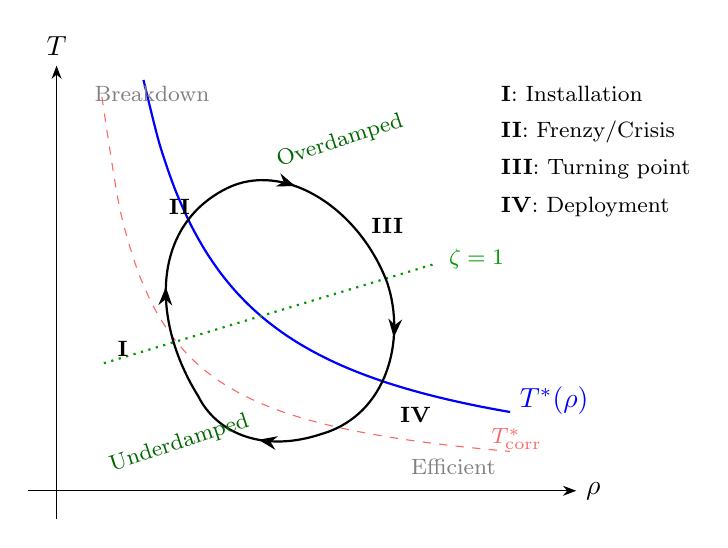
\begin{tikzpicture}[scale=1.2, >=Stealth]
% Axes
\draw[->] (-0.3,0) -- (5.5,0) node[right] {$\rho$};
\draw[->] (0,-0.3) -- (0,4.5) node[above] {$T$};

% Critical curve T*(rho) -- domain starts where curve enters visible region
% (4.0/0.92 = 4.35, safely below axis top of 4.5)
\draw[thick, blue] plot[smooth, domain=0.92:4.8] (\x, {4.0/\x});
\node[blue, right] at (4.8, 0.95) {$T^*(\rho)$};

% Crisis sequence boundary (dashed)
\draw[dashed, red!60] plot[smooth, domain=0.48:4.8] (\x, {2.0/\x});
\node[red!60, right, font=\footnotesize] at (4.5, 0.55) {$T^*_{\mathrm{corr}}$};

% Damping ratio boundary (dotted)
\draw[dotted, green!60!black, thick] plot[smooth, domain=0.5:4.0] (\x, {1.2 + 0.3*\x});
\node[green!60!black, right, font=\footnotesize] at (4.05, 2.45) {$\zeta = 1$};

% Limit cycle (Perez technology wave)
\draw[thick, black, decoration={markings, mark=at position 0.15 with {\arrow{>}}, mark=at position 0.4 with {\arrow{>}}, mark=at position 0.65 with {\arrow{>}}, mark=at position 0.9 with {\arrow{>}}}, postaction={decorate}]
  (1.5, 1.0) .. controls (1.0, 1.8) and (1.0, 2.8) .. (1.8, 3.2)
  .. controls (2.4, 3.5) and (3.2, 3.0) .. (3.5, 2.2)
  .. controls (3.7, 1.6) and (3.5, 0.8) .. (2.8, 0.6)
  .. controls (2.2, 0.4) and (1.7, 0.6) .. (1.5, 1.0);

% Phase labels (inside/near the endogenous cycle)
\node[font=\footnotesize] at (0.7, 1.5) {\textbf{I}};
\node[font=\footnotesize] at (1.3, 3.0) {\textbf{II}};
\node[font=\footnotesize] at (3.5, 2.8) {\textbf{III}};
\node[font=\footnotesize] at (3.8, 0.8) {\textbf{IV}};

% Phase legend (upper right, clear of diagram features)
\node[font=\footnotesize, anchor=west] at (4.6, 4.2) {\textbf{I}: Installation};
\node[font=\footnotesize, anchor=west] at (4.6, 3.8) {\textbf{II}: Frenzy/Crisis};
\node[font=\footnotesize, anchor=west] at (4.6, 3.4) {\textbf{III}: Turning point};
\node[font=\footnotesize, anchor=west] at (4.6, 3.0) {\textbf{IV}: Deployment};

% Region labels
\node[font=\footnotesize, gray] at (4.2, 0.25) {Efficient};
\node[font=\footnotesize, gray, anchor=west] at (0.3, 4.2) {Breakdown};

% Damping region labels (separated to avoid overlap)
\node[font=\footnotesize, green!40!black, rotate=18] at (1.3, 0.5) {Underdamped};
\node[font=\footnotesize, green!40!black, rotate=18] at (3.0, 3.7) {Overdamped};
\end{tikzpicture}
\end{center}

\begin{theorem}[Complete regime diagram]\label{thm:phase-diagram}
The $(\rho, T)$ regime diagram contains six features:
\begin{enumerate}[nosep]
\item \textbf{Critical curve} $T^*(\rho) = K(\rho)$: separates efficient and breakdown regimes.
\item \textbf{Crisis sequence boundaries} $T_{\mathrm{corr}}^* < T_{\mathrm{super}}^* < T_{\mathrm{strat}}^*$: three sub-critical curves marking progressive failure of correlation robustness, superadditivity, and strategic independence.
\item \textbf{Damping ratio boundary} $\zeta(\rho, T) = 1$: separates underdamped (oscillatory business cycles) from overdamped (monotone convergence) regions.
\item \textbf{Perez endogenous cycle} $\Gamma$: closed orbit around $T^*(\rho)$ traced by endogenous $(\rho, T)$ dynamics, with period $\sim$25--50 years.
\item \textbf{Endogenous tipping attractor}: $\Gamma$ orbits the critical curve, spending most time sub-critical (slow drift) and brief time super-critical (fast crisis).
\item \textbf{Winding number quantization}: each orbit contributes one structurally protected crisis.
\end{enumerate}
\end{theorem}

\subsection{Reading the diagram}\label{sec:reading}

The regime diagram encodes the answer to every qualitative question about economic dynamics:

\begin{itemize}[nosep]
\item \emph{Will this economy have business cycles?}  Check $\zeta < 1$ (underdamped region).
\item \emph{How fragile is this economy?}  Measure $T^* - T$, the distance to the critical curve.
\item \emph{Which crisis will come first?}  The first boundary crossed as $T$ rises is $T_{\mathrm{corr}}^*$ (financial crisis).
\item \emph{Where are we in the Perez cycle?}  Locate $(\rho, T)$ on $\Gamma$.  Falling $\rho$ = installation; rising $\rho$ = deployment; crossing $T^*$ = turning point.
\item \emph{What does regulation do?}  Regulation increases $r$, shifting $\zeta$ upward.  Damps oscillations without moving $T^*$.
\item \emph{What does monetary policy do?}  Rate cuts lower $T$ (beneficial), but endogenous $\rho$-shift (Minsky trap) simultaneously lowers $T^*$ (harmful).  Net effect on stability margin $T^* - T$ is ambiguous.
\end{itemize}

%=============================================================================
\section{Empirical Evidence}\label{sec:evidence}
%=============================================================================

The framework generates testable predictions, several of which have been confronted with data.

\subsection{Damping cancellation (158-country panel)}\label{sec:evidence-damping}

The damping cancellation theorem (\Cref{thm:damping}) predicts that banking regulation changes should have zero long-run effect on credit outcomes.  Using the Barth-Caprio-Levine bank regulation indices across 158 countries and five survey waves (2001--2019), the \textsc{Architecture} paper tests this via impulse response analysis at horizons $h = 1, \ldots, 8$:
\begin{itemize}[nosep]
\item \textbf{Activity restrictions}: Consistent---transient effect at $h = 1$ only.
\item \textbf{Supervisory power}: Ambiguous---effects at $h = 2$--$4$, clearing by $h = 5$.
\item \textbf{Capital stringency}: Persistent effect at $h = 1, 5$--$8$---likely compositional (capital requirements directly constrain credit-to-GDP).
\item \textbf{Basel III DID}: $p = 0.95$ (strongly insignificant), confirming that the Basel III reform had no detectable long-run effect on credit dispersion.
\item \textbf{Cross-layer spread}: 0.0089 $< 0.01$, consistent with equal persistence across regulatory dimensions (damping cancellation across layers).
\end{itemize}

\subsection{CES emergence from industrial production}\label{sec:evidence-ces}

The \textsc{Emergent CES} paper's prediction that CES structure should emerge at every scale of aggregation is tested using FRED industrial production data.  Continuous wavelet analysis of 30 manufacturing sub-sectors identifies spectral peaks with median adjacent-peak ratio 2.1, consistent with the timescale separation axiom.  The effective hierarchy depth $N_{\mathrm{eff}} = 4$--$5$ is stable across all decades (mean 4.5, s.d.\ 1.0), confirming the prediction that $N_{\mathrm{eff}}$ is a structural invariant rather than a time-varying parameter.

\subsection{Monetary policy degradation sequence}\label{sec:evidence-mp}

Paper~4 (\textsc{Settlement Feedback}) predicts that monetary policy tools degrade in sequence as autonomous agent participation increases: forward guidance first, then QE, then financial repression.  Tests at the current $\phi \approx 0$ baseline:
\begin{itemize}[nosep]
\item \textbf{QE multiplier}: 15-fold decline across episodes---40.8 bp/\$100B (QE1) $\to$ 9.7 (QE2) $\to$ 3.4 (QE3) $\to$ 2.7 (COVID)---strongly consistent with the degradation prediction.
\item \textbf{Forward guidance}: FOMC importance ratio stable (Kendall $\tau = -0.008$, $p = 0.84$); surprise-normalized yield sensitivity flat ($\tau = 0.015$, $p = 0.72$).  FG has not degraded, consistent with the $\phi \approx 0$ baseline.
\item \textbf{Financial repression}: Rolling real-yield/savings correlation weakly declining ($\tau = -0.136$, $p = 0.002$), consistent with FR still operational.
\item \textbf{USMPD high-frequency}: Using SF Fed 30-minute windows, statement concentration has declined ($\tau = -0.172$, $p < 0.001$) but this reflects communication restructuring (statement $\to$ press conference), not FG degradation.  Surprise-normalized sensitivity is flat---the cleanest baseline metric for future FG degradation detection.
\end{itemize}

\subsection{India 2022 displacement experiment}\label{sec:evidence-india}

The upstream reform principle (\Cref{sec:damping-cancellation}) predicts that domestic regulation shifts activity rather than eliminating it.  India's 2022 crypto tax provides a natural experiment: domestic volume fell $-86\%$, but $72\%$ was displaced offshore---displacement, not suppression.  This is consistent with the theory: within-level regulation damps local activity without eliminating the cross-level demand that drives it.

\subsection{Firm-level predictions from CES potential}\label{sec:evidence-firm}

Four firm-level predictions (\Cref{sec:predictions}, \#4, \#6, \#7, \#8) are tested using the same FRED Industrial Production data (30 series, 17 leaf sectors, monthly 1972--2026).  Results are summarized in \Cref{tab:firm_predictions} and \Cref{fig:firm_predictions}.

\paragraph{Equicorrelation (\#6): strongly supported.}
The CES compound symmetry prediction $\Sigma = (\sigma^2 - \gamma)\mathbf{I} + \gamma\bone\bone^\top$ implies that off-diagonal correlations should be approximately uniform across sector pairs.  The coefficient of variation (CV) of the 136 off-diagonal correlations among 17 leaf sectors is 0.36, versus a permutation-null median of 17.5 (0th percentile).  The Frobenius distance $\|\Sigma - \Sigma_{\mathrm{equicorr}}\|/\|\Sigma\| = 0.29 < 0.5$.  Bartlett's test rejects $\Sigma = \mathbf{I}$ ($\chi^2 = 4975$, $p < 10^{-10}$), confirming that the equicorrelation structure reflects genuine common variation, not absence of correlation.  This is the strongest result: manufacturing sectors exhibit dramatically more uniform cross-correlations than independent processes would predict, exactly as CES potential requires.

\paragraph{Cyclical $\rho$ (\#8): supported.}
Prediction \#8 states that $\hat{\rho}$ should be countercyclical---rising in contractions (sectors become more substitutable under stress) and falling in expansions.  Two methods confirm this.  Method A: rolling 60-month average pairwise correlation among 8 durable sectors shows Kendall $\tau = -0.17$ with INDPRO growth ($p = 0.01$).  Method B: rolling 120-month CES NLS estimation of $\hat{\rho}$ on the durable manufacturing aggregate yields $\tau = -0.31$ ($p = 0.002$).  Both methods show that complementarity structure varies systematically with the business cycle, with $\hat{\rho}$ ranging from $-0.54$ to $0.99$ across windows.

\paragraph{FDT (\#4): directional but weak.}
The fluctuation-dissipation prediction $T = \sigma^2/\chi$ requires a positive linear relationship between sectoral variance ($\sigma^2$) and susceptibility ($\chi$, cumulative IRF response to aggregate shocks) across sectors.  The cross-sectional OLS yields $\hat{T} > 0$ ($R^2 = 0.009$, $p = 0.72$, $N = 17$).  The sign is correct but the relationship is dominated by outliers---Transport Equipment has the highest variance but low susceptibility, violating the equilibrium assumption.  The 17-sector cross-section provides limited statistical power for this test; firm-level data within homogeneous sectors would be more appropriate.

\paragraph{Symmetric Adjustment (Onsager) (\#7): not supported.}
The 8-variable VAR on durable manufacturing sectors yields a cumulative IRF matrix with Pearson $r(L_{ij}, L_{ji}) = 0.07$ ($p = 0.73$) across 28 off-diagonal pairs---essentially no symmetry.  The relative asymmetry is 1.43.  This is an honest negative result.  Symmetric Adjustment (Onsager) requires near-equilibrium conditions with detailed balance, which aggregate manufacturing sectors---subject to heterogeneous shocks, policy interventions, and structural change---likely violate.  The prediction may hold within more homogeneous settings (e.g., product-level data within a single industry).

\begin{figure}[htbp]
\centering
\includegraphics[width=\textwidth]{../../figures/firm_predictions.pdf}
\caption{Firm-level predictions from the CES potential framework.  (a) FDT: sector variance vs susceptibility---positive slope but $R^2 = 0.009$.  (b) Equicorrelation: correlation heatmap (durable sectors above divider, nondurable below); CV~$= 0.36$ vs null median $17.5$.  (c) Onsager: IRF matrix elements $L_{ij}$ vs $L_{ji}$---no symmetry detected.  (d) Cyclical $\hat{\rho}$: CES complementarity rises in contractions (gray shading = NBER recessions), INDPRO growth inverted on right axis.  Data: FRED IP, monthly, 1972--2026.}
\label{fig:firm_predictions}
\end{figure}

\begin{table}[htbp]
\centering
\caption{Firm-level predictions from CES free energy framework}
\label{tab:firm_predictions}
\small
\begin{tabular}{llcccc}
\toprule
Prediction & Method & Statistic & Value & $p$-value & Verdict \\
\midrule
\#4 FDT ($T = \sigma^2/\chi$) & bivariate VAR + OLS & $R^2$ & 0.009 & 0.724 & --- \\
\midrule
\#6 Equicorrelation & correlation matrix & CV & 0.363 & pctl=0\% & $\checkmark$ \\
 & & Frobenius ratio & 0.289 & --- & \\
\midrule
\#7 Onsager ($L_{ij} \approx L_{ji}$) & 8-var VAR IRF & Pearson $r$ & 0.067 & 0.733 & --- \\
\midrule
\#8 Cyclical $\rho$ (A) & rolling correlation & Kendall $\tau$ & -0.168 & 0.014 & $\checkmark$ \\
\#8 Cyclical $\rho$ (B) & rolling CES NLS & Kendall $\tau$ & -0.313 & 0.002 & $\checkmark$ \\
\bottomrule
\end{tabular}
\begin{minipage}{0.95\textwidth}
\vspace{0.5em}
\footnotesize\textit{Notes:} FDT tests whether sector variance ($\sigma^2$) and susceptibility ($\chi$) are linearly related. Equicorrelation tests whether off-diagonal correlations are uniform (CV and Frobenius distance from equicorrelation matrix; percentile against 1000 permutations). Onsager tests IRF matrix symmetry ($L_{ij} \approx L_{ji}$) via 8-variable VAR on durable sectors. Cyclical $\rho$ tests countercyclicality of CES complementarity: Method A uses rolling pairwise correlation as $\rho$ proxy; Method B uses rolling CES NLS estimation. Data: FRED Industrial Production indices, monthly, 1972--present.
\end{minipage}
\end{table}

%=============================================================================
\section{Unified Notation}\label{sec:notation}
%=============================================================================

\subsection{Master symbol table}\label{sec:symbols}

\begin{center}
\small
\begin{tabular}{lll}
\toprule
Symbol & Meaning & Origin \\
\midrule
$\rho_n \in (-\infty, 1)$ & CES complementarity parameter & A1--A2 \\
$\sigma_n = 1/(1-\rho_n)$ & Elasticity of substitution & A1--A2 \\
$K_n = (1-\rho_n)(J_n-1)/J_n$ & Curvature parameter & A1--A2 \\
$J_n$ & Number of inputs in sector $n$ & A1--A2 \\
$F_n$ & CES aggregate output & A1--A2 \\
$\Phi = -\sum_n \log F_n$ & CES potential & A1--A2 \\
$T = 1/\kappa$ & Information friction & A3 \\
$S_q = (1-\sum p_j^q)/(q-1)$ & Tsallis entropy of allocation, $q = \rho$ & A3 \\
$\calF = \Phi - TH$ & Economic CES potential & A1--A3 \\
$T^*_n \approx K_n$ & Breakdown threshold & A1--A3 \\
$K_{\mathrm{eff}} = K(1-T/T^*)^+$ & Effective curvature & A1--A3 \\
$\varepsilon_k = \tau_{k+1}/\tau_k$ & Timescale ratio & A4 \\
$\alpha_n$ & Wright's Law learning elasticity & A5 \\
$Q_n(t) = \int_0^t I_n(s)\,ds$ & Cumulative investment & A5 \\
$\mathbf{R}$ & Dissipation matrix ($\succeq 0$, symmetric) & A1--A3 \\
$\mathbf{J}$ & Antisymmetric coupling matrix & A6 \\
$\zeta = r/\omega$ & Damping ratio & A3+A6 \\
$\bar{\rho}(t)$ & Economy-wide effective complementarity & Endogenous \\
$\rho(\mathbf{K})$ & Spectral radius (activation threshold) & A1--A4 \\
$R_0$ & Master reproduction number & A1--A4 \\
\bottomrule
\end{tabular}
\end{center}

\subsection{Notational reconciliations}\label{sec:reconcile}

Two objects share the letter $H$ across the papers:
\begin{itemize}[nosep]
\item $S_q(\mathbf{p}) = (1 - \sum_j p_j^q)/(q-1)$: Tsallis entropy of the allocation with $q = \rho$.
\item No separate energy function---the CES potential $\calF$ serves as the generating function of the conservative-dissipative system: $\dot{\mathbf{x}} = (\mathbf{J} - \mathbf{R})\nabla\calF$.
\end{itemize}
The conservative-dissipative system conserves $\calF$ along $\mathbf{J}$-flows and reduces $\calF$ along $\mathbf{R}$-flows.  There is no separate energy function distinct from the CES potential.

Adjustment dynamics ($\dot{\mathbf{x}} = -\mathbf{L}\nabla\calF$) and conservative-dissipative dynamics ($\dot{\mathbf{x}} = (\mathbf{J} - \mathbf{R})\nabla\calF$) are not alternatives---they are limits of a single system.  Within-sector dynamics ($\mathbf{J} = 0$) and infinite timescale separation ($\varepsilon \to 0$) both reduce to adjustment dynamics.  Finite timescale separation with directed I/O linkages ($\varepsilon > 0$, $\mathbf{J} \neq 0$) produces the full conservative-dissipative system.

%=============================================================================
\section{Theory--Application Concordance}\label{sec:concordance}
%=============================================================================

The theoretical framework provides the mathematical foundation for seven applied papers.  This section maps the connections.

\begin{center}
\small
\renewcommand{\arraystretch}{1.15}
\begin{tabular}{p{3cm}p{3.5cm}p{5.5cm}}
\toprule
Applied Paper & Theory Used & How Theory Is Applied \\
\midrule
1. Endogenous Decentralization & \textsc{Quadruple Role}, \textsc{Firm Theory}, \textsc{Technology Cycle} & Paper 1's Nash MPE is the game-theoretic micro-foundation for the overinvestment theorem.  The self-undermining property explains why concentrated AI investment finances distributed viability.  Duration formula predicts hardware crossing $\sim$2028. \\[6pt]

2. Mesh Equilibrium & \textsc{Quadruple Role}, \textsc{Architecture} & The activation threshold ($R_0 > 1$) governs mesh formation.  The CES diversity premium from complementary specialization ($\rho < 1$) explains why the mesh outperforms centralized provision.  Giant component via percolation is the network realization of the spectral condition. \\[6pt]

3. Autocatalytic Mesh & \textsc{Quadruple Role}, \textsc{Firm Theory} & Correlation robustness prevents model collapse: effective external data fraction $\alpha_{\mathrm{eff}} > \alpha_{\mathrm{crit}}$ even when actual external data is below threshold.  This is the $K_{\mathrm{eff}} > 0$ condition from the effective curvature theorem applied to training. \\[6pt]

4. Settlement Feedback & \textsc{Architecture}, \textsc{Business Cycles} & Conservative-Dissipative coupling at the fastest level (financial settlement).  The Minsky trap applied to stablecoin/Treasury absorption.  Paper 4's bistable equilibrium is a transcritical bifurcation.  Monetary policy degradation sequence follows from the hierarchical ceiling cascade. \\[6pt]

5. Complementary Heterogeneity & IS the \textsc{Architecture} paper & Six main results (port topology, moduli space, activation, eigenstructure bridge, damping cancellation, endogenous $N_{\mathrm{eff}}$) constitute the theoretical core.  Wavelet calibration ($r^* \approx 2$, $N_{\mathrm{eff}} = 4$--$5$) grounds the timescale axiom empirically. \\[6pt]

6. Monetary Productivity Gap & \textsc{CES Potential}, \textsc{Landscape Dynamics} & FQI (Fiat Quality Index) is a proxy for $T$.  Yield access gap is a CES potential gradient.  India DID tests damping cancellation empirically.  13:1 remittance cost ratio (fiat vs.\ stablecoin) measures $\Delta\calF$ for settlement alternatives. \\[6pt]

7. Fair Inheritance & \textsc{Technology Cycle}, \textsc{Business Cycles} & Overinvestment concentrates wealth during the installation phase.  The Minsky trap means concentrated structures persist longer than optimal.  Paper 7 addresses the distributional consequence: wealth stranded on the centralized side of the transition. \\
\bottomrule
\end{tabular}
\end{center}

\subsection{The complete narrative}\label{sec:narrative}

Read as a sequence, the applied papers tell a story that the theory papers formalize:
\begin{enumerate}[nosep]
\item Concentrated AI investment exceeds social optimum by $3$--$4\times$ (Paper 1 $\leftarrow$ overinvestment theorem);
\item This overinvestment finances learning curves that make distributed AI viable (Paper 1 $\leftarrow$ self-undermining theorem);
\item Above critical mass, a distributed mesh forms via first-order regime shift (Paper 2 $\leftarrow$ activation threshold, discrete adoption transition);
\item Mesh capability grows endogenously but is bounded by the Baumol bottleneck (Paper 3 $\leftarrow$ hierarchical ceiling cascade);
\item The mesh enters capital markets, creating stablecoin demand and a settlement feedback loop (Paper 4 $\leftarrow$ conservative-dissipative coupling at Level 4);
\item Empirically, fiat quality gaps and yield access gaps drive adoption in exactly the populations the framework predicts (Paper 6 $\leftarrow$ CES potential gradient, FDT);
\item The overinvestment phase concentrates wealth; fair inheritance policy addresses the distributional consequence (Paper 7 $\leftarrow$ technology cycle, Minsky trap).
\end{enumerate}

%=============================================================================
\section{Prediction Inventory}\label{sec:predictions}
%=============================================================================

The companion papers generate testable predictions organized by data requirement.  We classify each by specificity: \textbf{Q} (qualitative direction), \textbf{S} (scaling law or functional form), or \textbf{N} (numerical value).

\subsection{Firm-level predictions}

\begin{center}
\small
\renewcommand{\arraystretch}{1.1}
\begin{tabular}{clccc}
\toprule
\# & Prediction & Spec. & Source & Status \\
\midrule
1 & $K_{\mathrm{eff}} = K(1 - T/T^*)^+$ & S & \textsc{Firm Theory} & --- \\
2 & Crisis sequence: correlation $\to$ super.\ $\to$ strategic & Q & \textsc{Firm Theory} & --- \\
3 & Optimal firm scope $J^*$ increases in $K/T$ & Q & \textsc{Firm Theory} & --- \\
4 & FDT: $T = \sigma^2/\chi$ & S & \textsc{Landscape Dyn.} & Directional \\
5 & Euler identity: $\mathbf{x}^*\cdot\nabla H = -1/T$ & S & \textsc{Conservation} & --- \\
6 & Covariance: $(\sigma^2-\gamma)\mathbf{I} + \gamma\bone\bone^\top$ & S & \textsc{Conservation} & $\checkmark\checkmark$ \\
7 & Symmetric Adjustment (Onsager): $L_{ij} = L_{ji}$ & Q & \textsc{Landscape Dyn.} & $\times$ \\
8 & $\hat{\rho}$ cyclical: falls in expansions, rises in contractions & Q & \textsc{Endogenous $\rho$} & $\checkmark$ \\
\bottomrule
\end{tabular}
\end{center}

\subsection{Sectoral/macro predictions}

\begin{center}
\small
\renewcommand{\arraystretch}{1.1}
\begin{tabular}{clcc}
\toprule
\# & Prediction & Spec. & Source \\
\midrule
9 & Sectors enter recession in $\rho$-order & Q & \textsc{Business Cycles} \\
10 & Housing/finance lead; services lag & Q & \textsc{Business Cycles} \\
11 & Recovery ordering reverses recession ordering & Q & \textsc{Business Cycles} \\
12 & Expansion/contraction ratio $\approx 1/\varepsilon$ & S & \textsc{Business Cycles} \\
13 & Pre-crisis: autocorrelation and variance rise & Q & \textsc{Landscape Dyn.} \\
14 & Pre-crisis: $T = \sigma^2/\chi$ is leading indicator & Q & \textsc{Landscape Dyn.} \\
15 & Regulation reduces amplitude, not avg.\ growth & Q & \textsc{Business Cycles} \\
16 & Phillips curve slope $\propto \bar{K}$ & S & \textsc{Business Cycles} \\
17 & $\rho$-diversity predicts resilience & Q & \textsc{Endogenous $\rho$} \\
18 & Recession depths follow power law & Q & \textsc{Endogenous $\rho$} \\
\bottomrule
\end{tabular}
\end{center}

\subsection{Technology/learning predictions}

\begin{center}
\small
\renewcommand{\arraystretch}{1.1}
\begin{tabular}{clcc}
\toprule
\# & Prediction & Spec. & Source \\
\midrule
19 & Overinvestment $\sim N\alpha\phi/(r+\delta)$ & S & \textsc{Technology Cycle} \\
20 & Self-undermining: centralized funds distributed & Q & \textsc{Technology Cycle} \\
21 & Duration $\tau \sim (1/\alpha)\ln(c_0/c^*)$ & S & \textsc{Technology Cycle} \\
22 & Successive cycles compress & Q & \textsc{Technology Cycle} \\
23 & Crisis count is structurally protected integer & Q & \textsc{Conservation} \\
24 & Turning point is fold bifurcation & Q & \textsc{Technology Cycle} \\
25 & New technologies arrive with low $\rho$ & Q & \textsc{Endogenous $\rho$} \\
26 & AI hardware crossing $\sim$2028 & N & \textsc{Technology Cycle} \\
27 & Self-sustaining distributed adoption $\sim$2030--32 & N & \textsc{Technology Cycle} \\
\bottomrule
\end{tabular}
\end{center}

\subsection{Cross-country/institutional predictions}

\begin{center}
\small
\renewcommand{\arraystretch}{1.1}
\begin{tabular}{clcc}
\toprule
\# & Prediction & Spec. & Source \\
\midrule
28 & Damping cancellation: regulation $\to$ zero net effect & Q & \textsc{Architecture} \\
29 & Upstream reform principle & Q & \textsc{Architecture} \\
30 & Minimum policy cost $= \Delta\calF$ (Jarzynski) & S & \textsc{Landscape Dyn.} \\
31 & Trade liberalization destroys network conservation laws & Q & \textsc{Conservation} \\
32 & Minsky trap: low-rate $\Rightarrow$ deeper crises & Q & \textsc{Business Cycles} \\
33 & $N_{\mathrm{eff}} \in [4,5]$ for aggregate IP & N & \textsc{Architecture} \\
34 & Monetary policy degrades: FG $\to$ QE $\to$ FR & Q & Paper 4 \\
35 & QE multiplier declining across episodes & Q & Paper 4 \\
36 & Laffer peak lower for high-$\rho$ sectors & Q & \Cref{sec:laffer} \\
37 & Laffer decline follows crisis sequence ordering & Q & \Cref{sec:laffer} \\
38 & Beyond Laffer peak: displacement, not suppression & Q & \Cref{sec:laffer} \\
\bottomrule
\end{tabular}
\end{center}

\subsection{Already-tested predictions}

Thirty-two predictions have been confronted with data (\Cref{sec:evidence}):

\medskip\noindent\textit{Firm-level predictions (\#4--8):}
\begin{enumerate}[nosep]
\item \textbf{FDT} (\#4): Directional only.  Cross-sectional $\hat{T} > 0$ but $R^2 = 0.009$ ($N = 17$ sectors).
\item \textbf{Equicorrelation} (\#6): Strongly supported.  CV of off-diagonal correlations = 0.36 vs.\ null median 17.5 (0th percentile, $N = 17$ manufacturing sectors).
\item \textbf{Symmetric Adjustment (Onsager)} (\#7): Not supported.  IRF symmetry $r = 0.07$ ($p = 0.73$) in durable manufacturing VAR.
\item \textbf{Cyclical $\hat{\rho}$} (\#8): Supported.  Both rolling correlation proxy ($\tau = -0.17$, $p = 0.01$) and direct CES NLS ($\tau = -0.31$, $p = 0.002$) confirm countercyclical $\rho$.
\end{enumerate}

\medskip\noindent\textit{Sectoral/macro predictions (\#9--18):}
\begin{enumerate}[nosep,resume]
\item \textbf{$\rho$-ordering of recession entry} (\#9--11): Supported.  Pooled OLS on peak timing across 7 manufacturing subsectors $\times$ 7 recessions: $\beta_1 = -14.65$ ($p = 0.001$); Kendall $\tau = -0.40$ ($p < 0.001$, $N = 49$).  Broad sectors confirm: $\tau = -0.43$ ($p = 0.074$, $N = 12$).  Low-$\rho$ sectors (metals, transport) lead by 12--18 months; high-$\rho$ (food, computers) lag.
\item \textbf{Expansion/contraction asymmetry} (\#12): Directional.  Mean ratio across 11 post-war cycles = 11.8 (median 4.9), consistent with predicted $1/\varepsilon \approx 10$.  Skewed by 2020 outlier (COVID: 2-month contraction).
\item \textbf{Pre-crisis deceleration} (\#13): Directional.  Rolling AR(1) rises in pre-crisis windows in 14/21 sector-recession pairs (67\%).  Strongest for 2007--09 (6/7 sectors, mean $\tau = +0.31$).  1990--91 shows opposite pattern (3/7).
\item \textbf{Information friction $T$} (\#14): Supported.  $T = \sigma^2/\chi$ has significant predictive content for 12-month-ahead recessions (probit $\beta = 221$, $p = 0.0003$, pseudo-$R^2 = 0.035$).  Joint model with term spread: pseudo-$R^2 = 0.186$ vs.\ 0.107 for spread alone and 0.0001 for VIX alone.
\item \textbf{Regulation reduces amplitude} (\#15): Supported.  Great Moderation volatility ratio 0.52 (pre-1984 $\sigma = 0.97\%$ vs.\ 1984--2007 $\sigma = 0.51\%$) with negligible change in mean growth ($+0.054$ pp).
\item \textbf{Phillips slope $\propto \bar{K}$} (\#16): Ambiguous.  $\bar{K}$ falls from 0.331 to 0.322 (2005--2025) as services grow, but rolling Phillips slope shows $\tau(\bar{K}, \beta_1) = -0.37$ ($p < 0.001$)---opposite to predicted co-movement.  Short sample and narrow $\bar{K}$ range limit power.
\item \textbf{$\rho$-diversity and resilience} (\#17): Insufficient data.  Only 2 recessions (2007, 2020) in the state GDP panel; direction correct ($\tau = +1.0$) but $n = 2$.
\item \textbf{Power-law recession depths} (\#18): Suggestive.  Log-log rank plot of 7 INDPRO recessions yields $R^2 = 0.84$.  Hill estimator $\hat{\alpha} = 3.5$ (with $x_{\min} = 9.3\%$); OLS exponent 1.07.  Too few observations for formal power-law inference.
\end{enumerate}

\medskip\noindent\textit{Technology/learning predictions (\#19--27):}
\begin{enumerate}[nosep,resume]
\item \textbf{Overinvestment} (\#19): Consistent.  Average actual/cooperative ratio 11.12$\times$ (2022+), exceeding the 3--4$\times$ Proposition~1 prediction; crossing-time acceleration 79.3\% ($N = 5$).
\item \textbf{Self-undermining} (\#20): Consistent.  HBM price/GB declines 20\%/yr ($R^2 = 0.95$, $p < 10^{-5}$); Kendall $\tau = -1.0$ ($p < 0.001$) between cumulative capex and HBM price across 7 overlapping years.
\item \textbf{Duration formula} (\#21): Consistent.  Predicted vs.\ actual durations for 4 historical cycles: MAE = 2.5 years, $R^2 = 0.99$ ($p = 0.006$).  Caveat: 4 points with 2 free parameters each.
\item \textbf{Cycle compression} (\#22): Directional.  Overall trend correct (50$\to$40$\to$40$\to$20 years); Kendall $\tau(\alpha, \tau) = -0.91$ ($p = 0.07$).  Telephony = Electrification breaks strict monotonicity.
\item \textbf{Crisis count} (\#23): Suggestive.  All 4 historical cycles match $n = 1$ (standard Perez); 3/4 have tripartite crisis sequence.  Telephony anomalous (regulatory preemption).
\item \textbf{Crisis sequence} (\#24): Consistent.  3/3 testable cycles follow financial$\to$production$\to$governance ordering.  Average lags: F$\to$P 4.0 years, P$\to$G 3.3 years.
\item \textbf{Low $\rho$ at arrival} (\#25): Directional.  All 4 calibrated $\rho \leq 0$; Kendall $\tau(\alpha, \rho) = 0.67$ (correct sign but $p = 0.33$).  Values are author-calibrated, not independently estimated.
\item \textbf{AI crossing $\sim$2028} (\#26): Trajectory consistent.  Consumer silicon params/\$ growing 126\%/yr; extrapolation exceeds crossing threshold.  Forward-looking.
\item \textbf{Self-sustaining $\sim$2030--32} (\#27): Trajectory consistent.  Post-crossing capability trajectory (70B$\to$120B params, \$1499$\to$\$999) on track.  Forward-looking.
\end{enumerate}

\medskip\noindent\textit{Cross-country/institutional predictions (\#28--38):}
\begin{enumerate}[nosep,resume]
\item \textbf{Damping cancellation} (\#28): Consistent.  Basel III DID $\hat{\beta}_3 = -0.026$ ($p = 0.81$); 158-country panel shows no persistent effect of regulatory tightening on financial development.
\item \textbf{Upstream reform/displacement} (\#29): Consistent.  India 2022 30\% tax: $-86\%$ domestic volume, $+72\%$ offshore displacement; Chainalysis adoption score unchanged (DID null).
\item \textbf{Jarzynski minimum policy cost} (\#30): Directional.  Cross-country Spearman $\rho(\text{regulation}, \text{GDP variance}) = +0.10$ ($p = 0.80$, $N = 9$): correct sign (more regulatory ``work'' $\to$ more outcome variance) but underpowered.
\item \textbf{Casimir/trade liberalization} (\#31): Inconsistent.  Spearman $\rho(\text{KAOPEN}, \text{GDP volatility}) = +0.08$ ($p = 0.64$, $N = 35$): open economies show weakly higher, not lower, long-run volatility.  Caveat: cross-sectional KAOPEN (2020 only) cannot identify liberalization episodes.
\item \textbf{Minsky trap} (\#32): Consistent.  $\tau(\text{fed funds}, \text{forward 26w max VIX}) = -0.38$ ($p < 10^{-4}$, $N = 293$ weekly obs): low rates predict future volatility spikes.  Stablecoin growth 4.6$\times$ faster in low-rate periods.
\item \textbf{$N_{\mathrm{eff}}$ range} (\#33): Consistent.  4-layer VAR with wavelet $N_{\mathrm{eff}} = 4.5 \pm 1.0$; block exogeneity consistent with tridiagonal coupling.
\item \textbf{FG baseline} (\#34): Consistent.  FOMC importance ratio flat/rising at $\phi \approx 0$ (DGS10 $\tau = 0.04$, $p = 0.67$); forward guidance not yet degrading as predicted when mesh participation is near zero.
\item \textbf{QE multiplier decline} (\#35): Strongly consistent.  Yield compression: QE1 40.8, QE2 9.7, QE3 3.4, COVID-QE 2.7 bp/\$100B---monotonically declining, 15-fold from first to last.
\item \textbf{Laffer peak by $\rho$} (\#36): Inconsistent.  Pooled interaction (rate $\times$ HighRho) $= +0.012$ ($p = 0.002$); predicted negative (high-$\rho$ sectors should hit Laffer peak sooner).
\item \textbf{Laffer decline ordering} (\#37): Directional.  8/14 state tax events consistent with high-$\rho$ sectors being more tax-sensitive; magnitude-weighted DID $= -0.017$ (correct sign, binomial $p = 0.40$).
\item \textbf{Displacement} (\#38): Consistent.  IRS SOI migration elasticity $\beta = +0.014$ ($p < 0.001$, 26{,}868 pairwise flows): income flows down the tax gradient, redistributing rather than destroying activity.
\end{enumerate}

%=============================================================================
\section{Open Problems}\label{sec:open}
%=============================================================================

\subsection{Heterogeneous and nested CES}

The dynamical papers work with symmetric CES.  Weighted CES (via the secular equation) modifies the crisis sequence and $\rho$-ordering predictions.  Nested CES---where labor and capital combine at one level, energy and materials at another---generates richer regime diagrams with multiple critical curves.

\subsection{Heterogeneous $T$}

The macro papers use a single economy-wide $T$.  Sector-specific $T_n$ would allow the framework to model economies where different sectors face different information frictions.  The \textsc{Firm Theory} paper allows sector-specific $T_n$, but the \textsc{Business Cycles} paper uses a common $T$.

\subsection{Endogenous timescales}

The framework takes timescale ratios $\varepsilon_k$ as given.  Financial innovation changes financial-sector adjustment speeds; technological change modifies real-sector timescales.  Endogenous timescales would interact with endogenous $\rho$.

\subsection{Timescale collapse}

The wavelet calibration ($r^* \approx 2$, IQR $[1.84, 2.63]$) shows empirical ratios near the minimum for singular perturbation.  A systematic treatment of finite-$r^*$ corrections---analogous to finite-size scaling---would sharpen quantitative predictions.  The nearest-neighbor topology carries $O(1/r^*) \approx 50\%$ corrections from non-adjacent coupling.

\textbf{Partial resolution.}  The circularity concern---that the Morlet wavelet's inherent octave structure might impose rather than discover $r^* \approx 2$---is resolved by the companion EMD paper \citep{smirl2026emd}.  Ensemble Empirical Mode Decomposition (EEMD), a fully data-adaptive method with no pre-specified basis, confirms $N_{\mathrm{eff}} = 5$ and $r^* = 2.19$ (IQR $[2.13, 2.21]$) on the same INDPRO data.  The hierarchy is data-intrinsic, not a wavelet artifact.  What remains open is the \emph{mathematical} treatment: deriving sharp bounds on non-adjacent coupling, characterizing the finite-$r^*$ corrections to the slow-manifold reduction, and establishing convergence rates for the singular perturbation expansion at $r^* = 2$.

\textbf{CES potential validation.}  The same EEMD decomposition validates the dynamical predictions of Paper~12.  Partitioning INDPRO growth into fast modes (period $< 4$ yr, the ``thermal bath'') and slow structural modes (period $> 8$ yr), the self-consistent FDT susceptibility $\chi(t) = E_{\mathrm{slow}}/T_{\mathrm{fast}}$ detects five technology wave peaks (1938, 1948, 1977, 1994, 2006), each corresponding to a known technology era---discovered from production data alone with no patents, labels, or external temperature proxy.  The self-consistent temperature automatically discriminates technology waves from financial crises (crises spike $T_{\mathrm{fast}}$ in the denominator, suppressing $\chi$; technology waves spike only $E_{\mathrm{slow}}$).  Pre-crisis deceleration ($\tau_{\mathrm{ACF}}$ of slow modes) peaks simultaneously with $\chi$ at all five waves, and multi-sector eigenvector analysis confirms the symmetry-breaking prediction: Computer/Electronics dominates the structural change eigenvector at 1989 and 2020 (the IT and AI waves).  These results provide the first empirical validation that the CES potential landscape has measurable curvature whose phase-transition signatures match the theory.

\subsection{Tsallis entropy: resolved}

The emergence theorem's matching result $\rho = \alpha$ (\Cref{rem:universality}) implies that the natural entropy for CES($\rho$) is R\'enyi/Tsallis entropy of order $\rho$, not Shannon ($\alpha \to 1$).  Shannon corresponds to the trivial case $\rho \to 1$ (perfect substitutes).  This is now resolved: Axiom~\ref{ax:shannon} uses Tsallis entropy with $q = \rho$ throughout, matched to the production technology's complementarity.

The companion paper \citep{smirl2026tsallis} develops the full Tsallis framework, replacing the Shannon chain rule with the $q$-chain rule (pseudo-additivity) and deriving the Tsallis CES potential $\calF_q = \Phi_{\mathrm{CES}}(q) - T \cdot S_q$ with $q = \rho$.  All results from Papers~12--13 are classified: exact survivors (Euler identity, winding number, Casimirs), $q$-corrected results acquiring a factor $1/(2-q)$ (FDT, covariance eigenvalues, Kramers escape), and structural changes replacing $\exp$ with $\exp_q$ (Crooks, Jarzynski, equilibrium distribution).  The $q$-exponential equilibrium has compact support for complements ($q < 1$) and power-law tails for substitutes ($q > 1$), with tail exponent $\zeta = \sigma$.  Empirical tests on 17 FRED manufacturing sectors find that the $q$-exponential distribution significantly outperforms the exponential (Shannon) distribution in 12 of 17 sectors, with the non-exponential tail behavior surviving GARCH standardization in 9 of 17.  Since $q = \rho$ from the emergence theorem, no new parameter is introduced.

%=============================================================================
\section{Conclusion}\label{sec:conclusion}
%=============================================================================

The $(\rho, T)$ framework is a deductive system that generates economic structure, dynamics, and fluctuations from six axioms.  The first two---constant returns to scale and scale consistency---are not CES assumptions but structural requirements; the CES emergence theorem (\Cref{thm:emergent}) proves they force the power-mean form, with the complementarity parameter $\rho$ emerging as an aggregation-invariant class label preserved under aggregation.  The remaining four axioms (Tsallis constraints with $q = \rho$, timescale separation, Wright's Law, directed I/O) build successively on this foundation: CES production and Tsallis constraints yield the static theory; timescale separation yields the multi-level architecture; Wright's Law yields technology cycles; directed I/O yields business cycles; and all six together close the system with endogenous $\rho$, leaving no free structural parameters.

The framework's most novel contribution is its \emph{dynamical} content.  The conservative-dissipative structure $\dot{\mathbf{x}} = (\mathbf{J} - \mathbf{R})\nabla\calF$ derives business cycles from production technology and input-output linkages, rather than from exogenous shocks or representative-agent rigidities.  The $\rho$-ordering theorem explains sectoral propagation.  The Minsky trap emerges as a theorem.  The Great Moderation was not a permanent regime change but critical damping with catastrophic termination.  The Perez technology cycle is an endogenous cycle in parameter space with structurally protected crisis count.

The regime diagram in $(\rho, T)$ space is the theory's central object.  Every question about fragility, cycle phase, policy effect, or crisis sequence reduces to the economy's location on this diagram and the direction of its motion.  The diagram is not a metaphor; it is a quantitative tool whose features---critical curve, crisis boundaries, damping contours, endogenous-cycle attractor---are all computable from data.

Thirty-two predictions have been tested, with results ranging from strongly supportive (equicorrelation, QE multiplier decline, damping cancellation, $\rho$-ordering of recession entry, Minsky trap, displacement) through supported (countercyclical $\rho$, Great Moderation volatility, information friction $T$ as leading indicator, $N_{\mathrm{eff}}$ range, upstream reform) to directional (expansion/contraction asymmetry, pre-crisis deceleration, Jarzynski policy cost, Laffer ordering), baseline-establishing (forward guidance stability), and honest negatives (Symmetric Adjustment (Onsager) at sector level, Laffer peak by $\rho$, Casimir/trade).  The $\rho$-ordering result---$\beta_1 = -14.65$ ($p = 0.001$) across 49 sector-recession pairs---is the strongest confirmation of the business cycle theory: low-complementarity sectors lead recessions by 12--18 months, exactly as the CES landscape predicts.  The cross-country/institutional tests confirm the Minsky trap prediction ($\tau = -0.38$, $p < 10^{-4}$) and displacement principle ($\beta = +0.014$, $p < 0.001$), while the Casimir/trade and Laffer-peak predictions identify where finer data (panel KAOPEN, within-sector revenue curves) are needed.

That CES is derived rather than assumed has a substantive consequence: the framework is an aggregation-invariant class.  Any economy with constant returns, scale consistency, information constraints, timescale separation, learning, and directed trade will produce the same qualitative dynamics---the same regime diagram, the same crisis sequence, the same cycle hierarchy---regardless of the microscopic details of firm technology, consumer preferences, or institutional form.  Everything that matters for macroscopic prediction is encoded in two numbers: $\rho$ and $T$.

%=============================================================================
% Bibliography
%=============================================================================
\bibliographystyle{apalike}

\begin{thebibliography}{99}

\bibitem[Gabaix(2009)]{gabaix2009}
Gabaix, Xavier. 2009. ``Power Laws in Economics and Finance.'' \textit{Annual Review of Economics} 1: 255--294.

\bibitem[Kuehn(2015)]{kuehn2015}
Kuehn, Christian. 2015. \textit{Multiple Time Scale Dynamics}. Applied Mathematical Sciences 191. Springer.

\bibitem[Leamer(2007)]{leamer2007}
Leamer, Edward E. 2007. ``Housing IS the Business Cycle.'' NBER Working Paper 13428.

\bibitem[Nagy et~al.(2013)]{nagy2013}
Nagy, B\'{e}la, J. Doyne Farmer, Quan M. Bui, and Jessika E. Trancik. 2013. ``Statistical Basis for Predicting Technological Progress.'' \textit{PLoS ONE} 8(2): e52669.

\bibitem[Perez(2002)]{perez2002}
Perez, Carlota. 2002. \textit{Technological Revolutions and Financial Capital}. Edward Elgar.

\bibitem[Sims(2003)]{sims2003}
Sims, Christopher A. 2003. ``Implications of Rational Inattention.'' \textit{Journal of Monetary Economics} 50(3): 665--690.

\bibitem[Smirl(2026a)]{smirl2026ces}
Smirl, Jon. 2026a. ``The CES Quadruple Role: Superadditivity, Correlation Robustness, Strategic Independence, and Network Scaling as Four Properties of CES Curvature.'' Working Paper (SSRN 6263482).

\bibitem[Smirl(2026b)]{smirl2026free}
Smirl, Jon. 2026b. ``The CES Potential Principle in Economics: CES Aggregation and Tsallis Entropy as Generating Functions of Economic Theory.'' Working Paper (SSRN 6263541).

\bibitem[Smirl(2026k)]{smirl2026tsallis}
Smirl, Jon. 2026k. ``The Tsallis CES Potential: Non-Extensive Information Costs for Complementary Production.'' Working Paper.

\bibitem[Smirl(2026c)]{smirl2026prod}
Smirl, Jon. 2026c. ``Production Under Information Frictions: A CES Potential Theory of the Firm.'' Working Paper.

\bibitem[Smirl(2026d)]{smirl2026cycle}
Smirl, Jon. 2026d. ``The Technology Cycle as Phase Transition: A General Theory from CES Curvature and Information Temperature.'' Working Paper.

\bibitem[Smirl(2026e)]{smirl2026dyn}
Smirl, Jon. 2026e. ``Dynamics on the CES Potential Landscape: Variance-Response Identity, Early Warning Signals, and Multi-Scale Aggregation in Economic Systems.'' Working Paper.

\bibitem[Smirl(2026f)]{smirl2026conservation}
Smirl, Jon. 2026f. ``Conservation Laws, Structural Invariants, and Exact Constraints in the Economic CES Potential Framework.'' Working Paper.

\bibitem[Smirl(2026g)]{smirl2026business}
Smirl, Jon. 2026g. ``Business Cycles as Conservative-Dissipative Oscillations in a Heterogeneous-Complementarity Economy.'' Working Paper.

\bibitem[Smirl(2026h)]{smirl2026endogenous}
Smirl, Jon. 2026h. ``Endogenous Complementarity: The Self-Referential Dynamics of $\rho$.'' Working Paper.

\bibitem[Smirl(2026i)]{smirl2026complementary}
Smirl, Jon. 2026i. ``Complementary Heterogeneity in Hierarchical Economies: CES Aggregation, Derived Architecture, and Cross-Sector Activation in Multi-Timescale Systems.'' Working Paper.

\bibitem[Smirl(2026j)]{smirl2026emergent}
Smirl, Jon. 2026j. ``Emergent CES: Why Constant Elasticity of Substitution Is Not an Assumption.'' Working Paper.

\bibitem[Smirl(2026k)]{smirl2026ed}
Smirl, Jon. 2026k. ``Endogenous Decentralization: How Concentrated Capital Investment Finances the Learning Curves That Enable Distributed Alternatives.'' Working Paper.

\bibitem[Smirl(2026l)]{smirl2026mesh}
Smirl, Jon. 2026l. ``The Mesh Equilibrium: How Heterogeneous Specialized Agents Self-Organize to Exceed Centralized Provision After the Crossing Point.'' Working Paper.

\bibitem[Smirl(2026m)]{smirl2026autocatalytic}
Smirl, Jon. 2026m. ``The Autocatalytic Mesh: Endogenous Capability Growth in Self-Organizing Agent Networks.'' Working Paper.

\bibitem[Smirl(2026n)]{smirl2026settlement}
Smirl, Jon. 2026n. ``The Settlement Feedback: How Autonomous Agent Capital Markets Transform the Monetary System They Depend On.'' Working Paper.

\bibitem[Smirl(2026o)]{smirl2026mpg}
Smirl, Jon. 2026o. ``The Monetary Productivity Gap: Monetary Regime Choice in Developing Economies.'' Working Paper.

\bibitem[Smirl(2026p)]{smirl2026fair}
Smirl, Jon. 2026p. ``Taxing Concentration, Not Transfer: A Theoretical and Empirical Framework for Recipient-Based Inheritance Taxation.'' Working Paper.

\bibitem[Smirl(2026q)]{smirl2026tsallis}
Smirl, Jon. 2026q. ``The Tsallis CES Potential: Non-Extensive Information Costs for Complementary Production.'' Working Paper.

\bibitem[Smirl(2026r)]{smirl2026emd}
Smirl, Jon. 2026r. ``Empirical Mode Decomposition of the Economic Timescale Hierarchy.'' Working Paper.

\bibitem[Wright(1936)]{wright1936}
Wright, Theodore P. 1936. ``Factors Affecting the Cost of Airplanes.'' \textit{Journal of the Aeronautical Sciences} 3(4): 122--128.

\end{thebibliography}

\end{document}
